
%%%%%%%% ICML 2018 EXAMPLE LATEX SUBMISSION FILE %%%%%%%%%%%%%%%%%

\documentclass{article}
\usepackage[margin=1in]{geometry}
\usepackage{dblfloatfix}    % To enable figures at the bottom of page
% Recommended, but optional, packages for figures and better typesetting:
\usepackage{microtype}
\usepackage{graphicx}
%\usepackage{subfigure}
\usepackage{booktabs} \usepackage{stmaryrd}% for professional tables
\usepackage{stmaryrd}(
\usepackage[section]{placeins}
% hyperref makes hyperlinks in the resulting PDF.
% If your build breaks (sometimes temporarily if a hyperlink spans a page)
% please comment out the following usepackage line and replace
% \usepackage{icml2018} with \usepackage[nohyperref]{icml2018} above.
%\usepackage{hyperref}

% Attempt to make hyperref and algorithmic work together better:
\newcommand{\theHalgorithm}{\arabic{algorithm}}

\newcommand{\system}{\textsc{DreamCoder}~}
\newcommand{\systemEnding}{\textsc{DreamCoder}}
\newcommand{\lowerBound}{\mathscr{L}}
\newcommand{\denotation}[1]{{\llbracket #1 \rrbracket}}
\newcommand{\code}[1]{{\footnotesize\texttt{#1}}}
\newcommand{\scode}[1]{{\tiny\texttt{#1}}}
\newcommand{\codechar}[1]{{\footnotesize{\texttt{"#1"}}}}
% Use the following line for the initial blind version submitted for review:
%\usepackage[nohyperref]{icml2018}

\usepackage{xcolor}
\definecolor{pop1}{HTML}{1F78b4}
\definecolor{pop2}{HTML}{164C13}
\definecolor{pop3}{HTML}{d95F02}
\definecolor{orange}{HTML}{d95F02}
\definecolor{teal}{HTML}{1b9e77}
\newcommand{\pop}[1]{\textcolor{pop1}{#1}}
\newcommand{\popp}[1]{\textcolor{pop2}{#1}}
\newcommand{\tree}[1]{\textcolor{pop3}{#1}}
\newcommand{\orange}[1]{\textcolor{orange}{#1}}
\newcommand{\teal}[1]{\textcolor{teal}{#1}}

\newcommand{\greenCode}[1]{{\footnotesize\popp{\code{#1}}}}
\newcommand{\blueCode}[1]{{\footnotesize\pop{\code{#1}}}}

%\usepackage{hyperref}       % hyperlinks
\usepackage{url}            % simple URL typesetting
\usepackage{booktabs}       % professional-quality tables
\usepackage{amsfonts}       % blackboard math symbols
\usepackage{nicefrac}       % compact symbols for 1/2, etc.
\usepackage{microtype}      % microtypography
\usepackage{mathrsfs}
\usepackage{listings}
\usepackage{amsthm}
% use Times
\usepackage{times}
% For figures
\usepackage{graphicx} % more modern
%\usepackage{epsfig} % less modern
\usepackage{subfig} 
\usepackage{fancyvrb}


\usepackage{caption}
%\usepackage{subcaption}

\fvset{fontsize=\footnotesize}

\usepackage{amssymb}
\usepackage{listings}
\usepackage{wrapfig}
\usepackage{tabularx}


\usepackage{verbatim}
 \usepackage{booktabs}
 % For algorithms
\usepackage{algorithm}
%\usepackage{algorithmic}
\usepackage{algpseudocode}% http://ctan.org/pkg/algorithmicx
\usepackage{tikz}
\usepackage{circuitikz}
\usetikzlibrary{fit,bayesnet}
%\usetikzlibrary{arrows.meta}
%\usetikzlibrary{positioning}
%\usetikzlibrary{decorations.text}
\usetikzlibrary{decorations.pathmorphing}
\tikzset{squiggle/.style={decorate, decoration={snake,amplitude=.4mm}}}
\usepackage{dsfont}
\usepackage{amsmath}

\DeclareMathOperator*{\argmin}{arg\,min} % thin space, limits underneath in displays
\DeclareMathOperator*{\argmax}{arg\,max} % thin space, limits underneath in displays
 


% Packages hyperref and algorithmic misbehave sometimes.  We can fix
% this with the following command.

\newcommand{\Expect}{\mathds{E}} %{{\rm I\kern-.3em E}}
\newcommand{\indicator}{\mathds{1}} %{{\rm I\kern-.3em E}}
\newcommand{\expect}{\mathds{E}} %{{\rm I\kern-.3em E}}
\newcommand{\probability}{\mathds{P}} %{{\rm I\kern-.3em P}}
\newcommand{\shift}[1]{\uparrow^{#1}}
\newcommand{\substitute}[2]{[\$ #1 \mapsto #2]}
\newcommand{\reduce}{\longrightarrow}
\newcommand{\manyReduce}{\longrightarrow^*}

\newtheorem{definition}{Definition}



\begin{document}


\section{Introduction: Expertise}

Human learners acquire expertise in a wide range of domains: some of
us become experts in calculus, or cooking, or biology, music, tennis,
or software engineering, to name just a few, and every child develops
expertise in natural language, intuitive physics~\cite{Pete?},
intuitive psychology (theory-of-mind), and motor control.  This
picture contrasts sharply with the current state of machine
intelligence, where a machine is built to be an expert in a single
domain, like boardgames~\cite{alphaGo}, medical
diagnosis~\cite{mycin,CNNsForDiseaseDetection}, theorem
proving~\cite{eurisko}, or visual object recognition~\cite{alexNet}.
Thus an outstanding challenge in the long-term program of building
more humanlike machines is to develop an algorithm that, like people,
autonomously acquires expertise across many different kinds of
domains.

We contribute a model of the development of expertise that combines
two key ingredients.  First, an expert needs a sufficiently expressive
knowledge representation.  Following a long tradition in cognitive
science and AI, we represent knowledge as programs, which prior work
has used to represent expertise in recognition and generation of
handwriting and speech~\cite{lake2015human}, intuitive theories (of
kinship, taxonomy, etc.)~\cite{Ullman2012}, and natural language
grammar and
semantics~\cite{DBLP:journals/cogsr/SchmidK11,piantadosi2011learning}.
Second, atop this program representation, experts possess two kinds of
domain expertise.  They have at their disposal a powerful, yet
specialized, repertoire of concepts and abstractions: e.g., in
architecture, these are concepts like `arch' or `foundation'; in
software engineering these are libraries of code and domain-specific
languages (DSLs).  Here our model represents knowledge as programs,
and so we identify this kind of expertise with a DSL.  Experts also
have knowledge of when and how to deploy these domain-specific
concepts efficiently when solving new problems: e.g., mathematicians
efficiently search the space of proofs, intuiting which lemmas are
appropriate when; expert chefs intuit which compositions of
ingredients are likely tasty, before they actually start cooking.  For
our model, this aspect of expertise corresponds to the ability to
quickly assemble new, useful programs out of its DSL.

We integrate these ideas into a model called DreamCoder which acquires
expertise through a novel kind of wake/sleep or `dream' learning. The
model iterates through wake cycles -- where it solves problems by
writing programs -- and a pair of sleep cycles: a sleep cycle that
grows its DSL by replaying experiences from waking and consolidating
them into new abstractions, and a sleep cycle that improves its
knowledge of how to write programs by training a neural network on
replayed experiences as well as `dreams', or samples, from its DSL.

DreamCoder builds on multiple generations of AI research, going back
to the 1960's~\cite{solomonoff1964formal} when program-learning was
proposed as a paradigm for general AI.  Broadly speaking recent work
has either developed neural approaches for learning to efficiently
deploy a fixed
DSL~\cite{devlin2017robustfill,balog2016deepcoder,NGDS,spiral}, or
developed symbolic approaches for representing and searching through
spaces of
programs~\cite{gulwani2011automating,solar2008program,DBLP:books/daglib/0070933}.
We were motivated by approaches that learn or grow the
DSL~\cite{Dechter:2013:BLV:2540128.2540316,DBLP:conf/icml/LiangJK10,solomonoff1989system,DBLP:journals/corr/abs-1110-5667,stolle2002learning}.
Our goal with DreamCoder is to show that the combination of
neurally-guided search and DSL learning is a uniquely powerful way of
building systems that, like human learners, autonomously acquire the
expertise needed to navigate a new domain of problems.





\section{Introduction: AI/PL/dreaming}


An age-old dream within AI is a machine that learns and reasons by
writing its own programs.  This vision stretches back to the
1960's~\cite{solomonoff1964formal} and cuts to the core of much of
what it would take to build machines that learn and think like humans.
Computational models of cognition often explain the flexibility and
richness of human thinking in terms of program learning: from everyday
thinking and problem solving (motor program induction as an account of
recognition and generation of handwriting and
speech~\cite{lake2015human}; functional programs as a model of natural
language semantics~\cite{SOMETHING}) to learning problems that unfold
over longer developmental time scales: the child's acquisition of
intuitive theories (of kinship, taxonomy, etc.)~\cite{Ullman2012} and
natural language grammar~\cite{DBLP:journals/cogsr/SchmidK11}, to name
just a few.  An outstanding challenge, however, is to engineer
program-learners that display the same level of domain-generality as
the humans they are meant to model.

Recent program-learning systems developed within the AI and machine
learning community are impressive along many dimensions, authoring
programs for problem domains like drawing
pictures~\cite{spiral,ellis2017learning}, transforming
text~\cite{gulwani2011automating} and numerical
sequences~\cite{balog2016deepcoder}, and reasoning over common sense
knowledge bases~\cite{muggleton2015meta}.  These systems work in
different ways, but typically hinge upon a carefully hand-engineered
Domain Specific Language (DSL).  The DSL restricts the space of
programs to contain the kinds of concepts needed for one specific
domain.  For example, a picture-drawing DSL could include concepts
like circles and spirals, and a DSL for numerical sequences could
include sorting and reversing lists of numbers.  Modern systems also
learn how to efficiently deploy the DSL on new
problems~\cite{devlin2017robustfill,balog2016deepcoder,NGDS}, but --
unlike human learners -- do not discover the underlying system of
concepts needed to navigate the domain.

We contribute a program-induction system that learns the
domain-specific concepts (DSL) while jointly learning how to use those
concepts.  This joint learning problem models two complementary
notions of domain expertise: (1) domain experts have at their disposal
a powerful, yet specialized repertoire of concepts and abstractions
(analogous to the DSL) while also (2) having accurate intuitions about
when and how to use those concepts to solve new problems.

Our system is called DreamCoder because it acquires these two kinds of
expertise through a novel kind of wake/sleep or `dream'
learning~\cite{hinton1995wake}, iterating through a wake cycle --
where it solves problems by writing programs -- and a pair of sleep
cycles: a sleep cycle that grows the DSL by replaying experiences from
waking and consolidating them into new abstractions (modeled as
fragments of code), and a sleep cycle that improves its knowledge of
how to write programs by training a neural network based on replayed
experiences as well as `dreams', or samples, from the DSL.

DreamCoder builds on two lines of prior work.  One line of work
considers the problem of learning new concepts, abstractions, or
`options' from
experience~\cite{Dechter:2013:BLV:2540128.2540316,DBLP:conf/icml/LiangJK10,solomonoff1989system,DBLP:journals/corr/abs-1110-5667,stolle2002learning},
while the other line of work considers the problem of learning how to
deploy those concepts
efficiently~\cite{devlin2017robustfill,balog2016deepcoder,NGDS}.  Our
goal with DreamCoder is to show that the combination of these ideas is
uniquely powerful, and pushes us toward program-writing systems that,
like human learners, autonomously acquire the expertise needed to
solve a new class of problems.



\section{Introduction: NIPS}


Much of everyday human thinking and learning can be understood in
terms of program induction: constructing a procedure that maps inputs
to desired outputs, based on observing example input-output pairs.
People can induce programs flexibly across many different domains,
often from just one or a few examples.  For instance, if shown that a
text-editing program should map ``Jane Morris Goodall'' to
``J. M. Goodall'', we can guess it maps ``Richard Erskine Leakey'' to
``R. E. Leakey''; if instead the first input mapped to ``Dr. Jane'' or
``Goodall, Jane'', we might guess the latter should map to
``Dr. Richard'' or ``Leakey, Richard'', respectively.

The FlashFill system~\cite{gulwani2011automating} embedded in
Microsoft Excel solves problems such as these and is probably the best
known practical program-induction algorithm, but researchers in
programming languages and AI have had successes in many domains, such as handwriting recognition and
generation~\cite{lake2015human}, procedural
graphics~\cite{ellis2017learning,DBLP:journals/corr/abs-1804-01118}, question
answering~\cite{johnson2017clevr} and robot motion
planning~\cite{devlin2017neural}.  These systems
work in different ways, but most hinge upon a carefully engineered
\textbf{Domain Specific Language (DSL)}.  This is especially true for
systems like FlashFill that induce a wide range of programs
very quickly, in a few seconds or less.  DSLs constrain the search
over programs with strong prior knowledge in the form of a restricted
inventory of programming primitives finely tuned to the domain: for
text editing, these are operations like appending and
splitting on characters.

In this work, we consider the problem of building agents that learn to solve
program induction tasks, and also the problem of acquiring the prior knowledge
necessary to quickly solve these tasks in a new domain.  Representative problems
in three domains are shown in Table~\ref{initialExampleDSL}.  Our solution is an
algorithm that grows or boostraps a DSL while jointly training a neural network
to help write programs in the increasingly rich DSL.

\begin{table*}%[t!]
  \makebox[\textwidth][c]{
    \scriptsize
  \tabcolsep=4pt
  \renewcommand\code\texttt
  \renewcommand\codechar[1]{\texttt{"#1"}}
  \newcommand{\helpSize}{0.25cm}
  \begin{tabular}{>{\hspace{-0em}}c<{\hspace{-1em}}>{\hspace{-1em}}c<{\hspace{-1em}}>{\hspace{-2.5em}}c<{\hspace{-0.8em}}>{\hspace{-1em}}c<{\hspace{-1em}}}
    \toprule
    &{\normalsize List Functions}&{\normalsize Text Editing}&{\normalsize Symbolic Regression}\\\midrule
    \rotatebox[origin=c]{90}{\normalsize \pop{Programs} \& Tasks}&{\tabcolsep=7pt
      \begin{tabular}{cc}
        \begin{tabular}{c}
          \code{[7\, 2\, 3]}$\to $\code{[7\, 3]}         \\
          \code{[1\, 2\, 3\, 4]}$\to $\code{[3\, 4]} \\
          \code{[4\, 3\, 2\, 1]}$\to $\code{[4\, 3]} \\
          \pop{\code{$f(\ell) = $}\code{($f_1$ $\ell$ ($\lambda$ (x)}}\\
          \hspace{1.15cm}\pop{\code{(> x 2)))}}       \\
          \\
          \code{[2\, 7\, 8\, 1]}$\to $\code{8}               \\
          \hspace{0.15cm}\code{[3\, 19\, 14]}$\to $\code{19}                \\
          \pop{\code{$f(\ell) = $}\code{($f_2$ $\ell$)}}
        \end{tabular}
        &
        \hspace{-0.3cm}\begin{tabular}{c}
          \code{[7\, 3]}$\to $\code{False}                              \\
          \hspace{0.3cm}\code{[3]}$\to $\code{False}                    \\
          \hspace{-0.3cm}\code{[9\, 0\, 0]}$\to $\code{True\phantom{e}} \\
          \hspace{0.3cm}\code{[0]}$\to $\code{True\phantom{e}}                        \\
          \hspace{-0.3cm}\code{[0\, 7\, 3]}$\to $\code{True\phantom{e}}                \\
          \pop{\code{$f(\ell) = $}\code{($f_3$ $\ell$ 0)}}
        \end{tabular}
      \end{tabular}
    }
    &
    \hspace{-0.5cm}\begin{tabular}{c}
      +106 769-438$\to $106.769.438\\%&Nancy FreeHafer $\longrightarrow$ Dr. Nancy\\
      +83 973-831$\to $83.973.831\\
      \pop{$f(\text{\code{s}}) = $\code{(}$f_0$\code{  \codechar{.} \codechar{-}
      }}\\
      \hspace{1.25cm}\pop{\code{($f_0$ \codechar{.} \codechar{ }}}\\
      \hspace{1.4cm}\pop{\code{(cdr s)))}}\\
      ~\\
      Temple Anna H $\to $TAH\\
      Lara Gregori$\to $LG\\
      \pop{$f(\text{\code{s}}) = $\code{(}$f_2$\code{ s)}}\\
    \end{tabular}
    &
    \begin{tabular}{cc}
      
\includegraphics[width = 3em]{figures/functions/4.png}&
      
\includegraphics[width = 3em]{figures/functions/146}\\
      \pop{\code{$f($x$) = $($f_1$ x)}}&    \pop{\code{$f($x$) = $($f_6$ x)}}\\
      ~\\
      
\includegraphics[width = 3em]{figures/functions/112.png}&
        
\includegraphics[width = 3em]{figures/functions/92.png}
      \\
      \pop{\code{$f($x$) = $($f_4$ x)}}&    \pop{\code{$f($x$) = $($f_3$ x)}}\\

    \end{tabular}
    ~\\
    \midrule
    \rotatebox[origin=c]{90}{\normalsize \popp{DSL}}&
    \hspace{0cm}\begin{tabular}{l}
      % $f_0($\code{r}$,\ell) \,=\, $\code{(foldr $\ell$ r ($\lambda$ (x a)}\\
      % \phantom{$f_0($\code{r}$,\ell) \,=\, $\code{(foldr}}\code{(cons (index (length a) $\ell$) a)))}\\
      % \hspace{\helpSize}($f_1$: \emph{Get the largest number})\\
      % $f_0(\ell) \,=\, $\code{(foldr $\ell$ 0 ($\lambda$ (x a)}\\\hspace{0.8cm}\code{ (if (> a x) a x)))}\\
      % \hspace{\helpSize}($f_1$: \emph{Get the largest number in $\ell$})\\
      %NOTE: this is the actual invention, but I removed a redundant lambda
      % below: $f_0(\ell,$\code{r}$) \,=\, $\code{(foldr r $\ell$ ($\lambda$ (x a) (cons x a)))}\\
      %% \popp{$f_0(\ell,$\code{r}$) \,=\, $\code{(foldr r $\ell$ cons)}}\\
      %% \hspace{\helpSize}($f_0$: \emph{Append lists }\code{r}\emph{ and  $\ell$})\\
      \popp{$f_1(\ell,$\code{p}$) \,=\, $\code{(foldr $\ell$ nil ($\lambda$ (x a)}}\\
      \hspace{0.5cm}\popp{\code{(if (p x) (cons x a) a)))}}\\
      \hspace{\helpSize}($f_1$: \emph{Higher-order filter function})\\
      %(lambda (fold $0 0 (lambda (lambda (if (gt? $0 $1) $0 $1)))))
      \popp{$f_2(\ell) \,=\, $\code{(foldr $\ell$ 0 ($\lambda$ (x a)}}\\
      \popp{\phantom{$f_2(\ell) \,=\, $}\code{(if (> a x) a x)))}}\\
      \hspace{\helpSize}($f_2$: \emph{Maximum element in list $\ell$})\\
      \popp{$f_3(\ell,$\code{k}$) \,=\, $\code{(foldr $\ell$ (is-nil $\ell$)}}\\
      \phantom{$f_1(\ell,$}
      \popp{\code{($\lambda$ (x a) (if a a (= k x))))}}\\
      \hspace{\helpSize}($f_3$: \emph{Whether $\ell$ contains }\code{k})\\
    \end{tabular}&


  \hspace{0.5cm}\begin{tabular}{l}
    \popp{$f_0($\code{s}$,$\code{a}$,$\code{b}$) \,=\, $\code{(map ($\lambda$
    (x)}}\\
    \popp{\hspace{1cm}\code{ (if (= x a) b x)) s)}}\\
      \hspace{\helpSize}($f_0$: \emph{Performs character substitution)}\\
      \popp{$f_1($\code{s}$,$\code{c}$) \,=\, $\code{(foldr s s ($\lambda$ (x
      a)}\\\hspace{1.1cm}\popp{\code{ (cdr (if (= c x) s a))))}}}\\
        \hspace{\helpSize}($f_1$: \emph{Drop characters from }\code{s}\emph{ until  }\code{c}\emph{ reached})\\
      \popp{$f_2($\code{s}$) \,=\, $\code{(unfold s is-nil car
      }}\\
      \popp{\hspace{1cm}\code{($\lambda$ (z) (}$f_1$\code{ z \codechar{ })))}}\\
        \hspace{\helpSize}($f_2$: \emph{Abbreviates a sequence of words})\\
      %%   \popp{$f_3($\code{a}$,$\code{b}$) \,=\, $\code{(foldr a b cons)}}\\
      %% \hspace{\helpSize}($f_3$: \emph{Concatenate strings }\code{a}\emph{ and }\code{b})
  \end{tabular}&

  \begin{tabular}{l}
    \popp{$f_0($\code{x}$)\,=\,$\code{(+ x real)}}\\
    \popp{$f_1($\code{x}$)\,=\,$\code{($f_0$ (* real x))} }\\
    \popp{$f_2($\code{x}$)\,=\,$\code{($f_1$ (* x (}$f_0$\code{ x)))}}\\
    \popp{$f_3($\code{x}$)\,=\,$\code{($f_0$ (* x (}$f_2$\code{ x)))}}\\
    \popp{$f_4($\code{x}$)\,=\,$\code{($f_0$ (* x (}$f_3$\code{ x)))}}\\
    \hspace{\helpSize}\emph{($f_4$: 4th order polynomial)}\\
    \popp{$f_5($\code{x}$)\,=\,$\code{(/ real x)}}\\
    \popp{$f_6($\code{x}$)\,=\,$\code{($f_5$ ($f_0$ x))}}\\
    \hspace{\helpSize}\emph{($f_6$: rational function)}\\

  \end{tabular}
  \\\bottomrule\\
\end{tabular}}\vspace{-0.5cm}
\caption{Top: Tasks from three domains we apply our algorithm to, each followed by the programs \system discovers for them. Bottom: Several examples from learned DSL. Notice that learned DSL primitives can call each other, and that \system rediscovers higher-order functions like \code{filter} ($f_1$ under List Functions)}\label{initialExampleDSL}%\vspace{-0.5cm}
\end{table*}

Because any learning problem can in principle be cast as
program induction, it is important to delimit our focus.  In contrast
to computer assisted programming~\cite{solar2008program} or genetic
programming~\cite{DBLP:books/daglib/0070933}, our goal is not to automate software
engineering, or to synthesize large bodies of code starting from scratch.  Ours is a basic AI goal:
capturing the human ability to learn to think flexibly and efficiently
in new domains --- to learn what you need to know about a domain so you
don't have to solve new problems starting from scratch.  We are
focused on problems that people solve relatively
quickly, once they acquire the relevant domain expertise.  These
correspond to tasks solved by short programs --- if you have an
expressive DSL.  %% Even with a good DSL, program search may be
%% intractable;
%
% , and adding new library routines to the DSL only broadens the
% search space;
%
%% so we train a
%% neural network to guide the search procedure.

%\section{Overview of \system}

Our algorithm takes inspiration from several ways that skilled human
programmers have learned to code: Skilled coders build libraries of
reusable subroutines that are shared across related programming tasks,
and can be composed to generate increasingly complex and powerful
subroutines.  In text editing, a good library should support routines
for splitting on characters, but also specialize these routines to
split on particular characters such as spaces or commas that are
frequently used to delimit substrings across tasks.  Skilled coders
also learn to recognize what kinds of programming idioms and library
routines would be useful for solving the task at hand, even if they
cannot instantly work out the details.  In text editing, one might
learn that if outputs are consistently shorter than inputs, removing
characters is likely to be part of the solution; if every output
contains a constant substring (e.g., ``Dr.''), inserting or appending
that constant string is likely to be a subroutine.

Our algorithm is called \system because it is based on a
novel kind of ``wake-sleep'' learning (c.f. \cite{hinton1995wake}), iterating
between ``wake'' and ``sleep'' phases to achieve three goals: finding
programs that solve tasks; creating a DSL by discovering
and reusing domain-specific subroutines; and training a neural network
that efficiently guides search for programs in the DSL.
The learned DSL effectively encodes a prior on programs likely to
solve tasks in the domain, while the neural net looks at the example
input-output pairs for a specific task and produces a ``posterior''
for programs likely to solve that specific task.  The neural network
thus functions as a \textbf{recognition model} supporting a form of
approximate Bayesian program induction, jointly trained with a
\textbf{generative model} for programs encoded in the DSL, in the
spirit of the Helmholtz machine~\cite{hinton1995wake}. The
recognition model ensures that searching for programs remains
tractable even as the DSL (and hence the search space for programs)
expands.


%% Our \system
%% algorithm incorporates these insights by iterating
Concretely, our algorithm iterates through three phases. 
The \textbf{Wake} phase takes a given set of \textbf{tasks}, typically
several hundred, and searches for compact programs that solve these tasks,
guided by the current DSL and neural network.
The \textbf{Sleep-G} phase grows the DSL (or \textbf{G}enerative model),
which allows the agent to more compactly
write programs in the domain. We modify the structure of the DSL by
discovering regularities across programs, compressing
them to distill out common abstractions across  programs discovered during waking.\footnote{This is loosely biologically
    inspired by the formation of abstractions during sleep memory
    consolidation~\cite{DUDAI201520}}
The \textbf{Sleep-R} phase improves the search procedure by training a neural network (the \textbf{R}ecognition model) to
write programs in the current DSL, in the spirit of ``amortized'' or
``compiled'' inference~\cite{le2016inference}.
We train the recognition model on  two data sources: samples
from the DSL (as in the Helmholtz Machine's ``sleep'' phase), and
programs found during waking.%%  As the DSL
%% improves and as search finds more programs, the recognition model gets
%% both more data to train on, and better data.
\footnote{These two sources are also
    loosely biologically inspired by the distinct episodic replay and
    hallucination components of dream sleep~\cite{fosse2003dreaming}}
    

\textbf{Brisk overview of related work.} Prior work on program learning has largely assumed a fixed, hand-engineered DSL,
both in classic symbolic program learning approaches (e.g., Metagol:~\cite{muggleton2015meta},
FlashFill:~\cite{gulwani2011automating}),
neural approaches  (e.g., RobustFill:~\cite{devlin2017robustfill}), and hybrids of neural and
symbolic methods (e.g., Neural-guided deductive search:~\cite{ngds}, DeepCoder:~\cite{balog2016deepcoder}).
A notable exception is the EC algorithm~\cite{Dechter:2013:BLV:2540128.2540316},
which also learns a library of subroutines.
We find EC motivating, and go beyond it and other prior work through the following contributions: %% \begin{itemize}
%%   \setlength\itemsep{0}
%%   \item We show how to learn-to-learn programs in an expressive Lisp-like programming language;
%%   \item We give an algorithm for learning DSLs, built on a formalism known
%%     as Fragment Grammars~\cite{tim}; and 
%%   \item We give a hierarchical Bayesian framing of the problem that allows a
%%     joint inference of the DSL and recognition model.
%% \end{itemize}
\\\textbf{Contributions.} (1) We show how to learn-to-learn programs in an expressive Lisp-like programming language, including conditionals, variables, and higher-order recursive functions;
(2) We give an algorithm for learning DSLs,
built on a formalism known as Fragment Grammars~\cite{tim};
and (3) We give a hierarchical Bayesian framing enabling joint inference of the DSL and recognition model.
up

\section{The \system Algorithm}

 We first mathematically describe our 3-step algorithm as
 an inference procedure for a hierarchical Bayesian model (Section~\ref{mathematicalFraming}),
  and then describe each step algorithmically in detail (Section~\ref{explorationSection}-\ref{grammarInductionSection}).

 \subsection{Hierarchical Bayesian Framing}\label{mathematicalFraming}

\system takes as input a set of \textbf{tasks}, written $X$, each of which is a program synthesis problem.
It has at its disposal a domain-specific \emph{likelihood model}, written $\probability[x|p]$, which scores the likelihood of a task $x\in X$ given a program $p$.\footnote{For example, for string editing,
  the likelihood is 1 if the program predicts the observed outputs on the observed inputs,
  and 0 otherwise; when learning a generative model or probabilistic program, the likelihood is
the probability of the program sampling the observation.}
Its goal is to solve each of the tasks by writing a program,
and also to infer a DSL, written $\mathcal{D}$.
We equip $\mathcal{D}$ with a real-valued weight vector $\theta$, and together
$(\mathcal{D},\theta)$ define a generative model over programs.
We frame our goal as maximum a posteriori (MAP) inference of $(\mathcal{D},\theta)$ given $X$.
Writing $J$ for the joint probability of $(\mathcal{D},\theta)$ and $X$, we want the $\mathcal{D}^*$ and $\theta^*$ solving:
\begin{align}\label{intractableObjectives}
\nonumber  J(\mathcal{D},\theta)\triangleq \probability[\mathcal{D},\theta]&\prod_{x\in X} \sum_p \probability[x|p]\probability[p|\mathcal{D},\theta]\\
  \mathcal{D}^* = \argmax_{\mathcal{D}}\int J(\mathcal{D},\theta)\;\mathrm{d}\theta &\qquad
  \theta^* =\argmax_\theta J(\mathcal{D}^*,\theta)
\end{align}

%% Inference in this model is
%% difficult because the programs are unobserved,
%% and so we must solve a hard search problem to recover them. To make
%% search tractable we learn a bottom-up \emph{recognition
%%   model} (written $q(\cdot )$, Fig.~\ref{graphicalModel}(b)).
%% The recognition model $q(\cdot )$ is a neural
%% network that regresses from input/output pairs to a distribution over
%% programs likely to explain the input/outputs. We can also view $q(\cdot )$ as implementing an amortized
%% inference
%% scheme~\cite{le2016inference}.
%%  The neural recognition model and the
%% generative model embodied in the DSL jointly train each other, as they
%% iteratively learn to solve more programming tasks.



The above equations summarize the problem from the point of view of an ideal Bayesian learner.
However, Eq.~\ref{intractableObjectives}
is wildly intractable because evaluating $J(\mathcal{D},\theta)$ involves
summing over the  infinite set of all programs.
In practice we will only ever be able to sum over a finite set of programs.
So, for each task, we define a finite set of programs, called a \emph{frontier}, and only marginalize over the frontiers:
\\\noindent\textbf{Definition.} A \emph{frontier of task $x$}, written $\mathcal{F}_x$,
is a finite set of programs s.t. $\probability[x|p] > 0$ for all $p\in \mathcal{F}_x$.

Using the frontiers we  define the following intuitive lower bound on the joint probability, called $\lowerBound$:
\begin{align}
 J\geq \lowerBound\triangleq\probability[\mathcal{D},\theta]\prod_{x\in X} \sum_{p\in \mathcal{F}_x} \probability[x|p]\probability[p|\mathcal{D},\theta]
\end{align}
We alternate maximization of $\lowerBound$ w.r.t. $\left\{\mathcal{F}_x \right\}_{x\in X}$  (\textbf{Wake})
and $(\mathcal{D},\theta)$ (\textbf{Sleep-G}):


\\\noindent \textbf{Wake: Maxing $\lowerBound$ w.r.t.\ the frontiers.} Here $(\mathcal{D},\theta)$ is fixed and we
want to find new programs to add to  the frontiers so that $\lowerBound$ increases the most.
$\lowerBound$ most increases by finding programs where $\probability[x|p]\probability[p|\mathcal{D},\theta]\propto\probability[p|x,\mathcal{D},\theta]$ 
is large (i.e., programs with high posterior probability).
%Here we use a simple and generic enumerative program synthesis algorithm.
%% which we can accomplish by adding new programs to the frontiers means searching for new programs $p$ for task $x$
%% where  is large.
\\\noindent \textbf{Sleep-G: Maxing $ \lowerBound$ w.r.t.\ the DSL.} Here $\left\{\mathcal{F}_x \right\}_{x\in X}$ is held fixed, and so we can evaluate $\lowerBound$. Now the problem is that of searching the discrete space of DSLs and finding one maximizing $\int \lowerBound \;\mathrm{d}\theta$,
and then updating $\theta$ to $\argmax_\theta \lowerBound(\mathcal{D},\theta,\left\{\mathcal{F}_x \right\})$.
%To represent DSLs and search the space of DSLs, we use Fragment Grammars~\cite{tim}.

Searching for programs is hard because
of the large combinatorial search space. We ease this difficulty by training a neural recognition model, $q(\cdot |\cdot )$,
during the \textbf{Sleep-R} phase: $q$ is trained to approximate the
posterior over programs, $q(p|x)\approx \probability[p|x,\mathcal{D}]\propto\probability[x|p]\probability[p|\mathcal{D}}]$.
  Thus training the neural network amortizes the cost of finding programs with high posterior probability.

\textbf{Sleep-R: tractably maxing $\lowerBound$ w.r.t. the
  frontiers.}  Here we train %% a neural network, $q$, to predict a
%% distribution over programs conditioned on a task. The objective of $q$
%% is
$q(p|x)$ to assign high probability to programs $p$ where
$\probability[x|p]\probability[p|\mathcal{D},\theta]$ is large, because incorporating those programs
into the frontiers will most increase $\lowerBound$.

Intuitively, this 3-phase inference procedure can work in practice because each of the 3 phases bootstraps off of the others (Figure~\ref{feeding}). As the DSL grows and as the recognition model becomes more accurate, waking becomes more effective, allowing the agent to solve more tasks; when we solve more tasks during waking,
the Sleep-G phase has more data from which to learn the DSL; and, because Sleep-R is trained on both
samples from the DSL and programs found during waking,
the recognition model gets both more data, and higher-quality data, whenever the DSL improves and whenever we discover more successful programs.
\begin{figure}\centering
  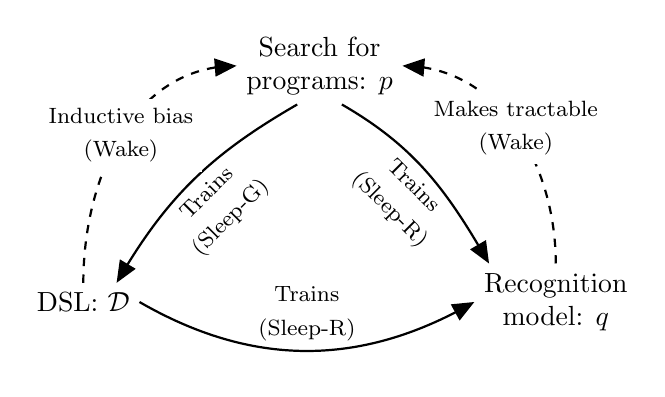
\begin{tikzpicture}
    \begin{scope}[shift = {(1,-1)}]
    \node[align = center](synthesis) at (6,4) {Search for \\programs: $p$};
    \node[align = center](DSL) at (3,1) {DSL: $\mathcal{D}$};
    \node[align = center](recognitionModel) at (9,1) {Recognition \\model: $q$};

    \draw [->,thick] (synthesis.-120) to[out = -150,in = 60] node[below,rotate = 45,align = center]{{\footnotesize Trains}\\{\footnotesize (Sleep-G)}} (DSL.30);
    \draw [->,thick] (synthesis.-60) to[out = -30,in = 120] node[below,rotate=-45,align = center]{{\footnotesize Trains}\\{\footnotesize (Sleep-R)}} (recognitionModel.150);
    \draw [->,thick] (DSL.east) to[out = -30,in = 210] node[above, align = center]{{\footnotesize Trains}\\{\footnotesize (Sleep-R)}} (recognitionModel.west);

    \draw [->,thick,dashed] (DSL.north) to[out = 90,in = 180] node[fill=white,align = center]{  \footnotesize{Inductive bias}\\\footnotesize{(Wake)}} (synthesis.west);
    \draw [->,thick,dashed] (recognitionModel.north) to[out = 90,in = 0] node[fill=white,align = center]{{\footnotesize Makes tractable}\\{\footnotesize (Wake)}} (synthesis.east);
  \end{scope}
    \end{tikzpicture}
  \caption{\system solves for programs, the DSL, and a recognition model. Each of these steps bootstrap off of the others in a Helmholtz-machine inspired wake/sleep inference algorithm.}  \label{feeding}
\end{figure}

\begin{figure}
  \begin{tikzpicture}
    \node at (0,0) (d){DSL};
    \node at ([yshift = -2cm]d) (t){$\text{Task}$};

    \node at ([xshift = 2cm]t) (nn){
      \begin{tikzpicture}[x=2.5cm,y=1.25cm,transform canvas={scale=0.2,shift={+(-1,2.5)}}]
        \tikzstyle{neuron}=[circle,fill=blue!50,minimum size=20pt]
        \fill[fill=white] (-0.25,-0.5) rectangle (2.25,-4.5);
        \node[rectangle] at (1,1) {};
        \foreach \name / \y in {1,...,4}
            \node[neuron] (I-\name) at (0,-\y) {};
        \foreach \name / \y in {1,...,3}
            \node[neuron] (H-\name) at (1,-\y-0.5) {};
        \foreach \name / \y in {1,...,4}
            \node[neuron] (O-\name) at (2,-\y) {};
        \foreach \source in {1,...,4}
            \foreach \dest in {1,...,3}
                \draw [-latex] (I-\source) -- (H-\dest);
        \foreach \source in {1,...,3}
            \foreach \dest in {1,...,4}
                \draw [-latex] (H-\source) -- (O-\dest);
      \end{tikzpicture}
    };
    \node[align = center, text width = 1cm] at ([yshift = 0.6cm]nn.north) {\baselineskip=0pt \small Recognition model\par};
    \draw [->] (t.east) -- ([xshift = -0.5cm]nn.west);

    \node[draw,rounded corners, inner sep = 10] at ([xshift = 4.2cm,yshift = -1cm]) (s){Search};
    \node at ([xshift=-7pt,yshift=5pt]s.north west) {$\mathcal{D}$};

    \draw [->] ([xshift = 0.5cm]nn.east) -- ([yshift = -0.25cm]s.west);
    \draw [->,rounded corners] (d.east) -- ([yshift = 2cm]nn.center) -- ([yshift = 0.25cm]s.west);

    \node[align=left] at (7,-1) (f) {Frontier\\{\small (set of programs)}};
    \draw [->  ] (s.east) -- (f.west);

    \draw [->  ,rounded corners] (t.south) -- ([yshift = -0.5cm]t.south) -- ([yshift = -0.5cm] s.south |- t.south) -- (s.south);
    \node at ([xshift = 0.5cm,yshift = -0.75cm]s.south) {Spec};

    \node at (4,-3.5) {\textbf{\textsc{Wake: Problem Solving}}};
    
    
  \end{tikzpicture}

  \vspace{1cm}
  
  

  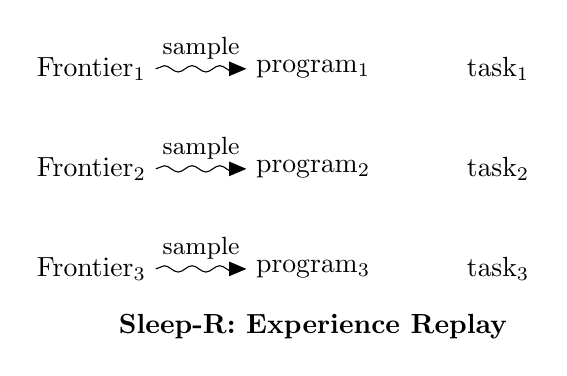
\begin{tikzpicture}
    \node at (0,0) (f1){Frontier$_1$};
    \node at ([yshift = -1cm]f1.south) (f2){Frontier$_2$};
    \node at ([yshift = -1cm]f2.south) (f3){Frontier$_3$};

    \node at ([xshift = 2cm]f1.east) (p1){program$_1$};
    \node at ([xshift = 2cm]f2.east) (p2){program$_2$};
    \node at ([xshift = 2cm]f3.east) (p3){program$_3$};


    \draw [->,squiggle ] (f1.east) -- node[above]{\small sample} (p1.west);
    \draw [->,squiggle ] (f2.east) -- node[above]{\small sample} (p2.west);
    \draw [->,squiggle ] (f3.east) -- node[above]{\small sample} (p3.west);
    
    \node at ([xshift = 1.5cm]p1.east) (t1){task$_1$};
    \node at ([xshift = 1.5cm]p2.east) (t2){task$_2$};
    \node at ([xshift = 1.5cm]p3.east) (t3){task$_3$};

    \node at ([yshift = -0.5cm]p3.south) {\textsc{\textbf{Sleep-R: Experience Replay}}};
  \end{tikzpicture}

  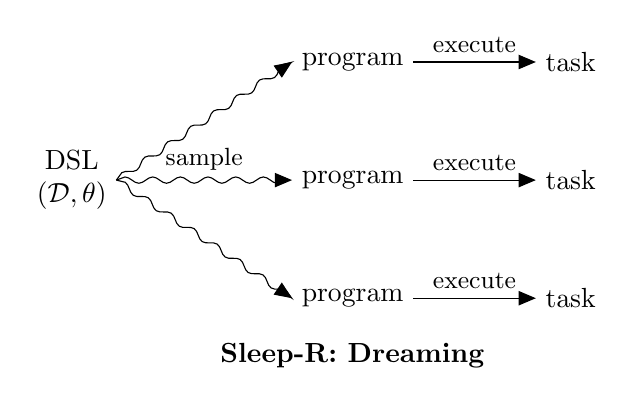
\begin{tikzpicture}
    \node[align=center] at (0,0) (d){DSL\\$(\mathcal{D},\theta)$};
    \node at ([xshift = 3cm]d.east) (p2){program};
    \node at ([yshift = 1.5cm]p2) (p1){program};
    \node at ([yshift = -1.5cm]p2) (p3){program};


    \draw[squiggle,-> ] (d.east) -- node[above]{\small sample} (p2.west);
    \draw[squiggle,-> ] (d.east) -- (p1.west);
    \draw[squiggle,-> ] (d.east) -- (p3.west);

    \node at ([xshift = 2cm]p1.east) (t1){task};
    \node at ([xshift = 2cm]p2.east) (t2){task};
    \node at ([xshift = 2cm]p3.east) (t3){task};
    \draw [-> ] (p1.east) -- node[above]{\small execute} (t1.west);
    \draw [-> ] (p3.east) -- node[above]{\small execute} (t3.west);
    \draw [-> ] (p2.east) -- node[above]{\small execute} (t2.west);

    \node at ([yshift = -0.5cm]p3.south) {\textsc{\textbf{Sleep-R: Dreaming}}};
  \end{tikzpicture}
  
  \vspace{2cm}
  
  \begin{tikzpicture}
    \node at (0,0) (f1){Frontier$_1$};
    \node at ([yshift = -1cm]f1.south) (f2){Frontier$_2$};
    \node at ([yshift = -0.7cm]f2.south) (ff){\textbf{$\vdots$}};
    \node at ([yshift = -1.2cm]f2.south) (ff){\textbf{$\vdots$}};
    \node at ([yshift = -1cm]ff.south) (f3){Frontier$_N$};

    \node(c)[rectangle, rounded corners, draw, minimum width = 3cm, minimum height = 6cm, anchor = north west] at (2,1) {};
    \node[anchor=north] at (c.north) {Compression};

    \draw [-> ] (f1.east) -- (c.west|-f1.east);
    \draw [-> ] (f2.east) -- (c.west|-f2.east);
    \draw [-> ] (f3.east) -- (c.west|-f3.east);

    \node[right](d) at ([xshift = 1.2cm,yshift = 0.7cm]c.east) {DSL $\mathcal{D}$};
    \node[right](t) at ([xshift = 1.2cm,yshift = -0.7cm]c.east) {Weights $\theta$};
    \draw [-> ] (c.east) -- (d.west);
    \draw [-> ] (c.east) -- (t.west);

    \node at (c.center) {
\begin{tikzpicture}[scale=0.7]
    %% \node[rotate=30] at (-2,0) {\begin{tabular}{c}
    %%     \footnotesize Program:\\
    %%     \code{($\lambda$ (x) (+ (- x) 1))}
    %% \end{tabular}};
    %\node at (,0.5) {\code{cons}};
%    \node [rotate=90] at (-2.3,-0.5) {\small program};
    
          \node(l1) at (0,0) {};
  \node[color=pop3](p1) at (-1,-1) {\code{+}};
  \node[color=pop3](n1) at (0.7,-0.9) {\code{1}};
  \node(x1) at (0,-1) {\code{1}};
  \draw[color=pop3] (l1.south) -- (p1.north);
  \draw[color=pop3] (l1.south) -- (n1.north);
  \draw[color=pop3] (-0.5,-0.45) -- (x1.north);

  \node(t) at (-0.5,0.5) {};
  \draw (l1.south) -- (t.south);
  \node(c) at (-1.5,-0.2) {\code{cons}};
  \draw (t.south) -- (c.north);
  
%    \draw  (l1.south) -- (-0.5,0.5);

  %% \node(c) at (-0.5,-1.5) {\code{-}};
  %% \node(z) at (0.5,-1.5) {\code{x}};

  %% \draw (0,-1) -- (c.north);
  %% \draw (0,-1) -- (z.north);
  
  \begin{scope}[shift={(-1,-2.5)}]
      \node(l1) at (0,0) {};
  \node[color=pop3](p1) at (-1,-1) {\code{+}};
  \node[color=pop3](n1) at (0.7,-0.9) {\code{1}};
  %\node(x1) at (0,-1) {};
  \draw[color=pop3] (l1.south) -- (p1.north);
  \draw[color=pop3] (l1.south) -- (n1.north);
  \draw[color=pop3] (-0.5,-0.45) -- (0,-1);


  \node(c) at (-0.5,-1.5) {\code{car}};
  \node(z) at (0.5,-1.5) {\code{z}};

  \draw (0,-1) -- (c.north);
  \draw (0,-1) -- (z.north);

%  \node [rotate=90] at (-2.3,-0.7) {\small program};
  
  \end{scope}

\begin{scope}[shift={(0,-5)}]
  \node[pop3](p1) at (-1,-1) {\code{+}};
  \node[pop3](n1) at (0.8,-0.7) {\code{1}};
  \node[pop3](a) at (0,-1) {\code{ }};
  %\node(x1) at (0,-1) {};
  \draw[pop3] (0,0) -- (p1.north);
  \draw[pop3] (0,0) -- (n1.north);
  \draw[pop3] (-0.55,-0.4) -- (a.north);
%  \node [rotate=90] at (-2.3,-0.7) {\small fragment};

  \end{scope}

\end{tikzpicture}
    };

    \node at ([yshift=-2.5cm,xshift = 4cm]c.south) {\textsc{\textbf{Sleep-G: Memory Consolidation}}};

    \end{tikzpicture}
  \end{figure}

\begin{figure}[h]
\centering
%  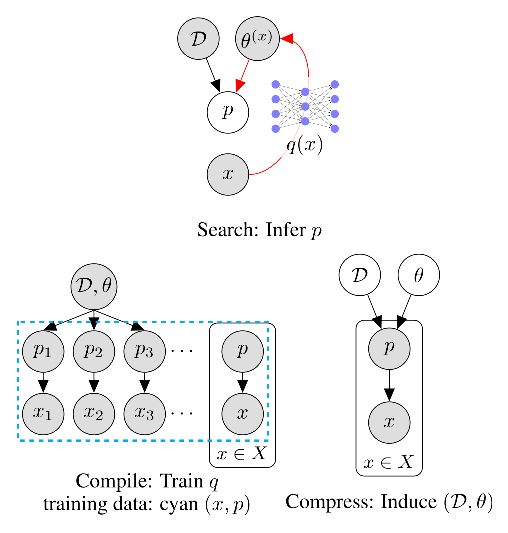
\includegraphics{figures/iterations.eps}
\begin{tikzpicture}
  \begin{scope}[shift={(2.5,0)}]
    \node[obs] at (3,3) (dx){$\mathcal{D}$};
    \node[latent] at (3.5,1.75) (zp){$p$};
%    \node[obs] at (4,3) (tx){$\theta^{(x)}$};
    \node[obs] at (3.5,0.7) (xp) {$x$};
    \node[align = center] at ([yshift = -0.6cm,xshift = 0.5cm]xp.south) {Wake: Infer $p$};
    \draw [->,red] (xp.east) to[out = 0,in = 90] node(nn){} (zp.north);
%    \draw [->,red] (tx) -- (zp);
    \draw [->] (dx) -- (zp);
    \node at (nn) {
      \begin{tikzpicture}[x=2.5cm,y=1.25cm,transform canvas={scale=0.2,shift={+(-1,2.5)}}]
        \tikzstyle{neuron}=[circle,fill=blue!50,minimum size=20pt]
        \fill[fill=white] (-0.25,-0.5) rectangle (2.25,-4.5);
        \node[rectangle] at (1,1) {};
        \foreach \name / \y in {1,...,4}
            \node[neuron] (I-\name) at (0,-\y) {};
        \foreach \name / \y in {1,...,3}
            \node[neuron] (H-\name) at (1,-\y-0.5) {};
        \foreach \name / \y in {1,...,4}
            \node[neuron] (O-\name) at (2,-\y) {};
        \foreach \source in {1,...,4}
            \foreach \dest in {1,...,3}
                \draw [-latex] (I-\source) -- (H-\dest);
        \foreach \source in {1,...,3}
            \foreach \dest in {1,...,4}
                \draw [-latex] (H-\source) -- (O-\dest);
      \end{tikzpicture}
    };
    \node[shift={+(0,-0.65)}] at (nn) [fill=white]{ $q(x)$ };
  \end{scope}

  \begin{scope}[shift={(0.7,-4.2)}]
    \node[obs] at (3,3) (dt){$\mathcal{D},\theta$};
    \node[obs] at ([yshift = -0.7cm,xshift = 0.0cm]dt.south) (p2){$p_2$};
    \node[obs] at ([yshift = -0.7cm,xshift = 0.0cm]p2.south) (x2){$x_2$};
    \draw [->] (p2.south) -- (x2.north);
    \draw [->] (dt.south) -- (p2.north);


    \node[obs] at ([yshift = 0cm,xshift = -0.5cm]p2.west) (p1){$p_1$};
    \node[obs] at ([yshift = -0.7cm,xshift = 0.0cm]p1.south) (x1){$x_1$};
    \draw [->] (p1.south) -- (x1.north);
    \draw [->] (dt.south) -- (p1.north);

    \node[obs] at ([yshift = 0cm,xshift = 0.5cm]p2.east) (p3){$p_3$};
    \node[obs] at ([yshift = -0.7cm,xshift = 0.0cm]p3.south) (x3){$x_3$};
    \draw [->] (p3.south) -- (x3.north);
    \draw [->] (dt.south) -- (p3.north);

    \node at ([yshift = 0cm,xshift = 0.3cm]p3.east) {$\cdots $};
    \node at ([yshift = 0cm,xshift = 0.3cm]x3.east) {$\cdots $};
      
    \node[obs] at ([yshift = 0cm,xshift = 1.3cm]p3.east) (zp){$p$};
    \node[obs] at ([yshift = 0cm,xshift = 1.3cm]x3.east) (xp) {$x$};
    \draw [->] (zp.south) -- (xp.north);
    \plate {}{(zp)(xp)}{$x\in X$};

    \draw[dashed,cyan,very thick] ([yshift = 0.5cm,xshift = -2]p1.west)
    rectangle  ([yshift = -0.45cm,xshift = +2]xp.east);
    \node[align = center] at ([yshift = -1cm,xshift = 0.6cm]x2.south) {Sleep-R: Train $q$\\training data: cyan $(x,p)$};
  \end{scope}
    
  \begin{scope}[shift={(7.7,-4)}]
    \node[latent] at (0.5,3) (d){$\mathcal{D}$};
    \node[latent] at (1.5,3) (t){$\theta$};
    \node[obs] at (1,1.75) (z){$p$};
%     \node[latent] at (3.5,1.5) (tx){$\theta^{(x)}$};
    \node[obs] at (1,0.5) (x) {$x$};
    \edge {z}{x};
    \edge {d,t}{z};
    \plate {}{(z)(x)}{$x\in X$};
    \node[align = center] at ([yshift = -1cm]x.south) {Sleep-G: Induce $(\mathcal{D},\theta)$};
  \end{scope}

\end{tikzpicture}
\end{figure}

\subsection{Wake: Searching for Programs}\label{explorationSection}

During waking, the agent's goal is to search for programs solving the tasks.  We use the simple approach of enumerating programs from
the DSL  in decreasing order of their probability according to the recognition model,
and then checking if a program $p$ assigns positive
probability to a task ($\probability[x|p] > 0$); if so, we incorporate $p$ 
into the frontier $\mathcal{F}_x$.

To make this concrete we need to define what programs actually are and
what form $\probability[p |\mathcal{D},\theta]$ takes.
We represent programs as $\lambda$-calculus expressions.
$\lambda$-calculus is a formalism for expressing functional programs
that closely resembles Lisp,
including variables, function application, and the ability to create new functions.
Throughout this paper we will write $\lambda$-calculus expressions in Lisp syntax.
Our programs are all strongly typed.
We use the Hindley-Milner polymorphic typing system~\cite{pierce} which is
used in functional programming languages like OCaml and Haskell.
%% Type variables are always written using lowercase Greek letters
%% and we write $\alpha\to \beta$ to mean a function that takes an input of type $\alpha$
%% and returns something of type $\beta$.
%% We use the notation $p:\tau$ to mean that the $\lambda$-calculus expression $p$
%% has the type $\tau$.
%% For example, to describe the type of the identity function
%% we would say \code{(lambda (x) x)}$:\alpha\to \alpha$.
%% We say a type $\alpha$ \emph{unifies} with $\tau$ if every expression
%% $p:\alpha$ also satisfies $p:\tau$. Furthermore, the act of \emph{unifying}
%% a type $\alpha$ with $\tau$ is to introduce constraints on the type
%% variables of $\alpha$ to ensure that $\alpha$ unifies with $\tau$.
%% See Supplement for more detail on program representation.
We now define DSLs:

\noindent\textbf{Definition: $(\mathcal{D},\theta)$.}
A DSL $\mathcal{D}$ is a set of typed $\lambda$-calculus expressions.
%\\\noindent\textbf{Definition.}
A weight vector $\theta$ for a DSL $\mathcal{D}$ is a vector of $|\mathcal{D}| + 1$ real numbers:
one number for each DSL element $e\in \mathcal{D}$, written $\theta_e$ and controlling the probability of  $e$ occurring in a program,
and a weight controlling the probability of a variable occurring in a program, $\theta_{\text{var}}$.

Together with its weight vector,
a DSL defines a distribution over programs, $\probability[p|\mathcal{D},\theta]$.
In the supplement, we define this distribution  
by specifying a procedure for drawing samples from $\probability[p|\mathcal{D},\theta]$.
Care must be taken to ensure that programs are well-typed
 and that variable scoping rules are obeyed.
%% With this distribution in hand, we search for programs by enumerating
%% $\lambda$-calculus expressions in decreasing order of their probability under
%% $(\mathcal{D},\theta)$.


Why enumerate, when the program synthesis community has invented many
sophisticated algorithms that search for programs?~\cite{solar2008program,schkufza2013stochastic,feser2015synthesizing,osera2015type,polozov2015flashmeta}.
We have two reasons:
(1) A key point of our work is that learning the DSL, along with a neural recognition model, can make program induction tractable, even if the search algorithm is very simple.
(2) Enumeration is a general approach that can be applied to any program induction problem. Many of these more sophisticated approaches require special conditions on
  the space of  programs.

  However, a drawback of   enumerative search  is that we have no
efficient means of solving for arbitrary constants that might occur in a
program. In Sec.~\ref{regressionSection},
we will show how to find programs with real-valued constants
by automatically differentiating through the program and setting the constants using gradient descent.
%% In Sec.~\ref{textSection}
%% we will show that the bottom-up neural recognition model can learn
%% which discrete constants should be included in a program.







\subsection{Sleep-R: Training a Neural Recognition Model}\label{recognitionSection}

The purpose of training the recognition model is to amortize the cost
of searching for programs.  It does this by learning to predict, for
each task, programs with high likelihood according to
$\probability[x|p]$ while also being probable under the prior
$(\mathcal{D},\theta)$.  Concretely, the recognition model $Q$
predicts, for each task $x\in X$, a distribution over programs,
$Q(\cdot |x)$.
We want $Q(\cdot |x)$ to approximate the posterior $\probability[\cdot |x,\mathcal{D},\theta]$.

\subsubsection{Training $Q$}
How should we get the data to train $q$?
This is nonobvious  because we are considering a weakly supervised setting (i.e., learning only from tasks and not from (program, task) pairs).
One approach is to sample programs from the DSL,
run them to get their input/outputs,
and then train $q$ to predict the program from the input/outputs.
This is like how a Helmholtz machine
trains its recognition model during its ``sleep'' phase~\cite{dayan1995helmholtz}.
The advantage of ``Helmholtz machine'' training is that
we can draw unlimited samples from the DSL,
training on a large amount of data.
Another approach is
 self-supervised learning,
training $q$ on the (program, task)
pairs discovered during waking.
The advantage of self-supervised learning
is that the training data is much higher quality,
because we are training on the actual tasks.
Due to these complementary advantages,
we train on both these sources of data.

Formally, $q$ should approximate the true posteriors over programs: minimizing the expected KL-divergence, $  \expect\left[\text{KL}\left(\probability[p|x,\mathcal{D},\theta]\|q(p|x) \right) \right]$,
 equivalently maximizing $  \expect[\sum_p\probability[p|x,\mathcal{D},\theta]\log q(p|x) ]$,
%% \begin{equation*}
%%   \expect\left[\sum_p\probability[p|x,\mathcal{D},\theta]\log q(p|x) \right]
%% \end{equation*}
 where the expectation is taken over tasks. Taking this expectation over the empirical distribution of tasks gives self-supervised training; taking it over samples from the generative model gives  Helmholtz-machine style training.
 The  objective for a recognition model ($\mathcal{L}_{\text{RM}}$) combines the Helmholtz machine ($\mathcal{L}_{\text{HM}}$) and self supervised ($\mathcal{L}_{\text{SS}}$) objectives:
 \begin{align}
   \mathcal{L}_{\text{RM}} &= \mathcal{L}_\text{SS} + \mathcal{L}_\text{HM}\\
\nonumber\mathcal{L}_{\text{HM}} &= \expect_{(p,x)\sim(\mathcal{D},\theta) }\left[\log q(p|x)\right]\\
\nonumber\mathcal{L}_{\text{SS}} &= \expect_{x\sim X}\left[\sum_{p\in \mathcal{F}_x}
  \frac{\probability\left[x,p|\mathcal{D},\theta \right]}{\sum_{p'\in \mathcal{F}_x}\probability\left[x,p'|\mathcal{D},\theta \right]}\log q(p|x)\right]
\end{align}

  The $\mathcal{L}_{\text{HM}}$ objective is essential for data efficiency:
all of our experiments train \system on only a few hundred tasks, which is too little for
a high-capacity neural network $q$.
Once we bootstrap a $(\mathcal{D},\theta)$,
we can draw unlimited samples from $(\mathcal{D},\theta)$
and train $q$ on those samples.

Evaluating $\mathcal{L}_{\text{HM}}$ involves sampling programs from
the current DSL, running them to get their outputs,
and then training $q$ to regress from the input/outputs to the program.
Since these programs map inputs to outputs,
we need to sample the inputs as well.
Our solution is to sample the inputs
from the empirical observed distribution of inputs in $X$.

\subsubsection{Parameterizing $Q$}

Broadly the literature contains two different approaches to
parameterizing conditional distributions over programs.  The first
approach, seen in systems like RobustFill~\cite{devlin2017robustfill}
and~\cite{zavershynskyi2018naps}, is to use a recurrent neural network
to predict the program token-by-token ala Seq2Seq or Seq2Tree.  The
advantage of this approach is that the neural net can predict the
entire program, so if the network is sufficiently powerful, it can
completely solve the synthesis problem.  There are two disadvantages
to this approach.  First, these models perform poorly at out-of-sample
generalization~\cite{}, which is critical for our setting, as the
agent may need to solve new tasks that are qualitatively different
from the tasks it has solved so far.  Second, a powerful deep
recurrent network may be costly to sample or enumerate from ---
so if the network cannot easily solve a task, we cannot compensate
with rapid sampling or enumeration.  In contrast, state-of-the-art
enumerative program synthesizers evaluate millions of programs per
second~\cite{feser2015synthesizing}.

The second approach is to have $Q$ predict a fixed-dimensional weight
vector, which then biases a fast enumerator~\cite{balog2016deepcoder}
or sampler~\cite{menon2013machine}.  This approach can enjoy strong
out-of-sample generalization, because it can fall back on enumeration
or sampling when the target program is unlike the training programs.
A main drawback is that the neural net is deliberately handicapped,
and can only send so much information about the target program.

We adopt a middle ground between these two extremes.  Our recognition
model predicts a distribution over primitives in the DSL,
conditioned on the local context in the syntax tree of the
program. When predicting the next node to add to the syntax tree of a program,
the recognition model
conditions on the parent node, as well as
which argument is being generated.
This is a kind of `bigram' model over trees,
where the bigrams
take the form of (parent, child, argument index).
See Figure~\ref{bg}.
This parameterization
has three main advantages:
(1) it supports fast enumeration
and sampling of programs,
because the
recognition model
only needs to run once for each task;
(2) it allows the recognition model to provide fine-grained
information about the structure of the target program;
and (3)
training this recognition model
causes it to learn to break symmetries in the space of programs,
described next.
\begin{figure}
\centering  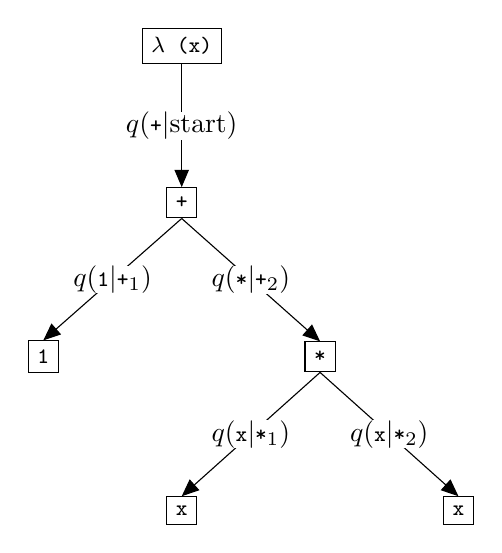
\begin{tikzpicture}%[every node/.style={inner sep=0,outer sep=0}]
    \node(l)[draw] at (0,0) {\code{$\lambda$ (x)}};
    \node(k)[draw] at ([yshift=-50]l.south) {\code{+}};
    \node(o)[draw] at ([xshift=-50,yshift=-50]k.south) {\code{1}};
    \node(m)[draw] at ([xshift=50,yshift=-50]k.south) {\code{*}};
    \node(x1)[draw] at ([xshift=50,yshift=-50]m.south) {\code{x}};
    \node(x2)[draw] at ([xshift=-50,yshift=-50]m.south) {\code{x}};

    \draw[->] (l.south)-- node[fill=white,align=center,midway,inner sep=0,outer sep=0]{$q(\code{+}|\text{start})$}(k.north);
    \draw[->] (k.south)--node[fill=white,align=center,midway,inner sep=0,outer sep=0]{$q(\code{1}|\code{+}_1)$}(o.north);
    \draw[->] (k.south)--node[fill=white,align=center,midway,inner sep=0,outer sep=0]{$q(\code{*}|\code{+}_2)$}(m.north);
    \draw[->] (m.south)--node[fill=white,align=center,midway,inner sep=0,outer sep=0]{$q(\code{x}|\code{*}_2)$}(x1.north);
    \draw[->] (m.south)--node[fill=white,align=center,midway,inner sep=0,outer sep=0]{$q(\code{x}|\code{*}_1)$}(x2.north);
\end{tikzpicture}
\caption{Parameterization of distribution over programs predicted by recognition model.
  Here the program (syntax tree shown above) is \code{($\lambda$ (x) (+ 1 (* x x)))}.
Each conditional distribution predicted by the recognition model is written $q(\text{child}|\text{parent}_{\text{argument index}})$.}
  \end{figure}

\subsection{Sleep-G: Learning a Generative Model (a DSL)}\label{grammarInductionSection}

The purpose of the DSL is to
offer a set of abstractions
that allow an agent to easily express solutions to the tasks at hand.
Intuitively, we want the algorithm to look at the programs found
during waking and generalize beyond them, both so the DSL can better
express the current solutions, and also so that the DSL might expose
new abstractions which will later be used to discover more programs.
Formally, we want the DSL maximizing $\int \lowerBound\;\mathrm{d}\theta$ (Sec.~\ref{mathematicalFraming}).
We replace this marginal with an AIC approximation, giving the following objective for DSL induction:
\begin{align}
\nonumber      \log \probability[\mathcal{D}]& + 
\argmax_{\theta}\Bigg(\log \probability[\theta|\mathcal{D}] - \|\theta\|_0 \\&+\sum_{x\in X}\log \sum_{p\in \mathcal{F}_x}\probability[x|p]\probability[p|\mathcal{D},\theta]\Bigg)
\label{AIC}
\end{align}
At a high level, our approach is to search locally through the space
of DSLs, proposing small changes to $\mathcal{D}$ until Eq.~\ref{AIC}
fails to increase.  These small changes consist of introducing new
candidate $\lambda$-expressions into the DSL.

However, there is a snag with this simple approach:
whenever we add a new expression $e$ to the DSL,
the programs found during waking ($\left\{\mathcal{F}_x \right\}$)
are not written in terms of $e$.
Concretely, imagine we wanted to discover a new DSL procedure for doubling numbers,
after having found the programs
\code{(cons (+ 9 9) nil)} and \code{($\lambda$ (x) (+ (car x) (car x)))}.
As human programmers,
we can look at these pieces of code and recognize that,
if we define a new procedure called \code{double},
defined as \code{($\lambda$ (x) (+ x x))},
then we can rewrite the original programs as
\code{(cons (double 9) nil)} and \code{($\lambda$ (x) (double (car x)))}.
This process is a kind of refactoring
where a new subroutine is defined (\code{double})
and the old programs rewritten
in terms of the new subroutine.
Figure~\ref{mapFactor}
diagrams this refactoring
process for a more complicated
setting,
where the agent must rediscover the higher-order function \code{map}
starting from the basics of Lisp and the Y-combinator.

Formally, we want a DSL
which puts high probability on
any refactoring of the programs found during waking, maximizing:
\begin{align}
\nonumber      \log \probability[\mathcal{D}]& + 
\argmax_{\theta}\Bigg(\log \probability[\theta|\mathcal{D}] - \|\theta\|_0 \\&+\sum_{x\in X}\log \sum_{p\in \mathcal{F}_x}\probability[x|p]\max_{p'\manyReduce p}\probability[p'|\mathcal{D},\theta]\Bigg)
\label{factorObjective}
\end{align}
where $p'\manyReduce p$
is the standard notation for ``expression $p'$ evaluates to $p$ by the rules of $\lambda$-calculus''~\cite{pierce}.

Equation~\ref{factorObjective} captures the idea that we want
to add new components to the DSL while jointly refactoring our old
programs in terms of these new components.  But
this joint inference problem is intractable, because there are
infinitely many ways of refactoring a program.
We combine two ideas to make this refactoring process tractable:

\textbf{Idea 1:} Limit the degree to which
a piece of code can be refactored.
Instead of considering every refactoring,
bound the number of $\lambda$-calculus evaluation steps
separating a refactoring from its original program.
Formally,
we define the set of $n$-step refactorings as:
\begin{equation}
  R_n(p) = \left\{p'\;:\;p'\underbrace{\reduce p''\reduce\cdots\reduce}_{\text{$\leq n$ times}} p \right\}
\end{equation}
where $p_1\reduce p_2$ is the standard notation for ``$p_1$ rewrites to $p_2$
in one step according to the rules of $\lambda$-calculus''~\cite{pierce}.
For example,
\begin{align*}
  \code{((lambda (x) (x x)) (lambda (y) y))}\reduce&\\
  \code{((lambda (y) y) (lambda (y) y))}\reduce&\\
  \code{(lambda (y) y)}&
\end{align*}
Returning to Equation~\ref{factorObjective},
this approximation gives the following objective:
\begin{align}
\nonumber      \log \probability[\mathcal{D}]& + 
\argmax_{\theta}\Bigg(\log \probability[\theta|\mathcal{D}] - \|\theta\|_0 \\+&\sum_{x\in X}\log \sum_{p\in \mathcal{F}_x}\probability[x|p]\max_{p'\in R_n(p)}\probability[p'|\mathcal{D},\theta]\Bigg)
\label{limitedObjective}
\end{align}
In practice, setting the number of refactoring steps $n$ to 3 suffices
to give a competent DSL learning algorithm.  Although the number of
refactorings is now finite, it is still prohibitively large, and in
fact grows exponentially quickly both as a function of $n$ and as a
function of the size of the program being refactored.  For example,
for the programs in Figure~\ref{mapFactor}, there are approximately
$10^{14}$ possible refactorings.  Next, we show how to tame this
exponential explosion.

\textbf{Idea 2:} Rather than explicitly enumerate every refactoring,
we developed a technique for compactly representing and efficiently
calculating the set of all refactorings.  The key idea is to represent
the set of refactorings using a \emph{version
  space}~\cite{lau2001programming,mitchell1977version,polozov2015flashmeta}.
A version space is a tree-shaped data structure
that compactly represents a large set of programs.
We first define version spaces over $\lambda$-calculus expressions,
and then give a dynamic program for constructing a version space
that represents the set of possible refactorings (i.e., $R_n(p)$).
This technique is astronomically more efficient than
explicitly representing
the space of possible refactorings:
for the example in Figure~\ref{mapFactor},
we represent
the space of refactorings using a version space with
$10^6$ nodes,
which encodes $10^{14}$ refactorings.
Formally, a version space is either:
\begin{itemize}
\item A deBuijn\footnote{deBuijn indices are an alternative way of naming variables in $\lambda$-calculus. When using deBuijn indices, $\lambda$-abstractions are written \emph{without} a variable name, and variables are written as the count of the number of $\lambda$-abstractions up in the syntax tree the variable is bound to. For example, $\lambda x.\lambda y. (x\;y)$ is written $\lambda\lambda (\$1\;\$0)$ using deBuijn indices. See~\cite{pierce} for more details.} index: written $\$i$, where $i$ is a natural number
\item An abstraction: written $\lambda v$, where $v$ is a version space
\item An  application: written $(f \;x)$, where both  $f$ and $x$ are version spaces
\item A  union: $\uplus V$, where $V$ is a set of version spaces
\item The empty set, $\varnothing$
\item The set of all $\lambda$-calculus expressions, $\Lambda$
\end{itemize}
The purpose of a version space to compactly represent a set of programs.
We refer to this set as the \textbf{extension} of the version space:
\begin{definition}
  The \textbf{extension} of a version space $v$ is written $\denotation{v}$
  and is defined recursively as:
  \begin{align*}
    \denotation{\$i}& = \left\{\$i \right\}\\
    \denotation{\lambda v}& = \left\{\lambda e : e\in \denotation{v} \right\}\\
    \denotation{(v_1\; v_2)}& = \left\{(e_1\;e_2) : e_1\in \denotation{v_1},\;e_2\in \denotation{v_2} \right\}\\
    \denotation{\uplus V}& = \left\{e : v\in V,\;e\in \denotation{v} \right\}\\
    \denotation{\varnothing}& = \varnothing\\
    \denotation{\Lambda}& = \Lambda
    \end{align*}
\end{definition}
Version spaces also support efficient membership checking, which we
write as $e\in v$, and which is equivalent to $e\in \denotation{v}$.
Important for our purposes, it is also efficient to refactor the
members of a version space's extension in terms of a new DSL.
We define $\textsc{refactor}(v|\mathcal{D})$ inductively as:
\begin{align}
  \textsc{refactor}(v|\mathcal{D}) &= \begin{cases}
    e\text{, if $e\in \mathcal{D}$ and $e\in v$. Exploits the fact that $e\in v$ can be efficiently computed.}\\
    \textsc{refactor}'(v|\mathcal{D})\text{, otherwise.}
  \end{cases}\label{FACTORING}\\\nonumber
  \textsc{refactor}'(e|\mathcal{D})& = e\text{, if $e$ is a leaf}\\\nonumber
  \textsc{refactor}'(\lambda b|\mathcal{D}) &= \lambda \textsc{refactor}(b|\mathcal{D})\\\nonumber
  \textsc{refactor}'(f\;x|\mathcal{D}) &= \textsc{refactor}(f|\mathcal{D})\;\textsc{refactor}(x|\mathcal{D})\\\nonumber
  \textsc{refactor}'(\uplus V|\mathcal{D}) &= \argmin_{e\in \left\{\textsc{refactor}(v|\mathcal{D})\;:\;v\in V \right\}}\text{size}(e|\mathcal{D})\nonumber
  \end{align*}
where $\text{size}(e|\mathcal{D})$ for program $e$ and DSL $\mathcal{D}$
is the size of the syntax tree of $e$,
when members of $\mathcal{D}$ are counted as having size 1.
Concretely, $  \textsc{refactor}(v|\mathcal{D})$ calculates $\argmin_{p\in \denotation{v}}\text{size}(p|\mathcal{D})$.

In Appendix~\ref{appendixVersion}, we describe a dynamic program for
efficiently constructing a version space containing every $n$-step
refactoring.
This dynamic program, which we call $I\beta^n(p)$,
satisfies $\denotation{I\beta^n(p)} =  R_n(p)$.
In other words,
this dynamic program
builds a data structure
that represents the entire set of
refactorings -- but without having to explicitly enumerate all of the refactorings.

With this machinery in hand, we now have all the pieces needed to
learn a DSL (Algorithm~\ref{grammarInductionAlgorithm}).
To define the prior distribution over $(\mathcal{D},\theta})$ (Algorithm~\ref{grammarInductionAlgorithm}, lines 7-8), we penalize the syntactic complexity of the $\lambda$-calculus expressions in the DSL, defining $    \probability[\mathcal{D}]\propto\exp(-\lambda\sum_{p\in \mathcal{D}}\text{size}(p) )$ where $\text{size}(p)$  measures the size of the syntax tree of program $p$,
  and $\lambda$ controls how strongly we regularize the size of the DSL.
  We place a symmetric Dirichlet prior over the weight vector $\theta$.

To appropriately score each proposed $\mathcal{D}$ we must reestimate
 the weight vector $\theta$ (Algorithm~\ref{grammarInductionAlgorithm}, line 7).
Although this  may seem 
very similar to estimating the parameters of a probabilistic context free grammar,
for which we have effective approaches like the Inside/Outside algorithm~\cite{international2000derivation},
our DSLs are context-sensitive due to the presence of variables
in the programs and also due to the polymorphic typing system.
Appendix~\ref{mapAppendix} derives a tractable MAP estimator for $\theta$.



\begin{algorithm}%[H]
  %\setcounter{algorithm}{2} % there are two algorithms in the main paper.
  \caption{DSL Induction Algorithm}
  \label{grammarInductionAlgorithm}
  \begin{algorithmic}[1]
    \State {\bfseries Input:} Set of frontiers $\{\mathcal{F}_x\}$
    %         \STATE \textbf{Hyperparameters:} Pseudocounts $\alpha$, regularization parameter $\lambda$
    \State \textbf{Output:} DSL $\mathcal{D}$, weight vector $\theta$
    \State $\mathcal{D}\gets$ every primitive in $\{\mathcal{F}_x\}$
    \While{true}         
    \State $\forall p\in \bigcup_{x}\mathcal{F}_x: $ $v_p\gets I\beta_n(p)$ \Comment{Construct a version space for each program}
    \State Define $L(\mathcal{D}',\theta) =  \prod_x \sum_{p\in \mathcal{F}_x} \probability[x|p]\probability[\text{\textsc{refactor}}(p|\mathcal{D}')|\mathcal{D}',\theta]$ \Comment{Likelihood if $(\mathcal{D}',\theta)$ were the DSL}
    \State Define $\theta^*(\mathcal{D}') = \argmax_\theta \probability[\theta|\mathcal{D}'] L(\mathcal{D}',\theta)$ \Comment{MAP estimate of $\theta$}
    \State Define $\text{score}(\mathcal{D}') = \log \probability[\mathcal{D}'] + L(\mathcal{D}',\theta^*) - \|\theta\|_0$ \Comment{objective function}
    \State components $\gets$ $\left\{\textsc{refactor}(v|\mathcal{D})\;:\;\forall x, \forall p\in \mathcal{F}_x, \forall v\in \text{children}(v_p) \right\}$ \Comment{Propose many new DSL components}
    \State proposals $\gets$ $\left\{\mathcal{D}\cup\left\{c \right\}\;:\;\forall c\in \text{components} \right\}$ \Comment{Propose many new DSLs}
    \State $\mathcal{D}'\gets \argmax_{\mathcal{D}'\in \text{proposals}}\text{score}(\mathcal{D}') $\Comment{Get highest scoring new DSL}
    \State \textbf{if }$\text{score}(\mathcal{D}') < \text{score}(\mathcal{D})$\textbf{ return }$\mathcal{D},\theta^*(\mathcal{D})$\Comment{No changes to DSL led to a better score}
    \State $\mathcal{D}\gets\mathcal{D}'$ \Comment{Found better DSL. Update DSL.}
    \State $\forall x\;:\;\mathcal{F}_x\gets\left\{\text{\textsc{refactor}}(p|\mathcal{D})\;:\; p\in \mathcal{F}_x\right\}$\Comment{Refactor frontiers in terms of new DSL}
    \EndWhile
  \end{algorithmic}
\end{algorithm}




\begin{figure*}
  \centering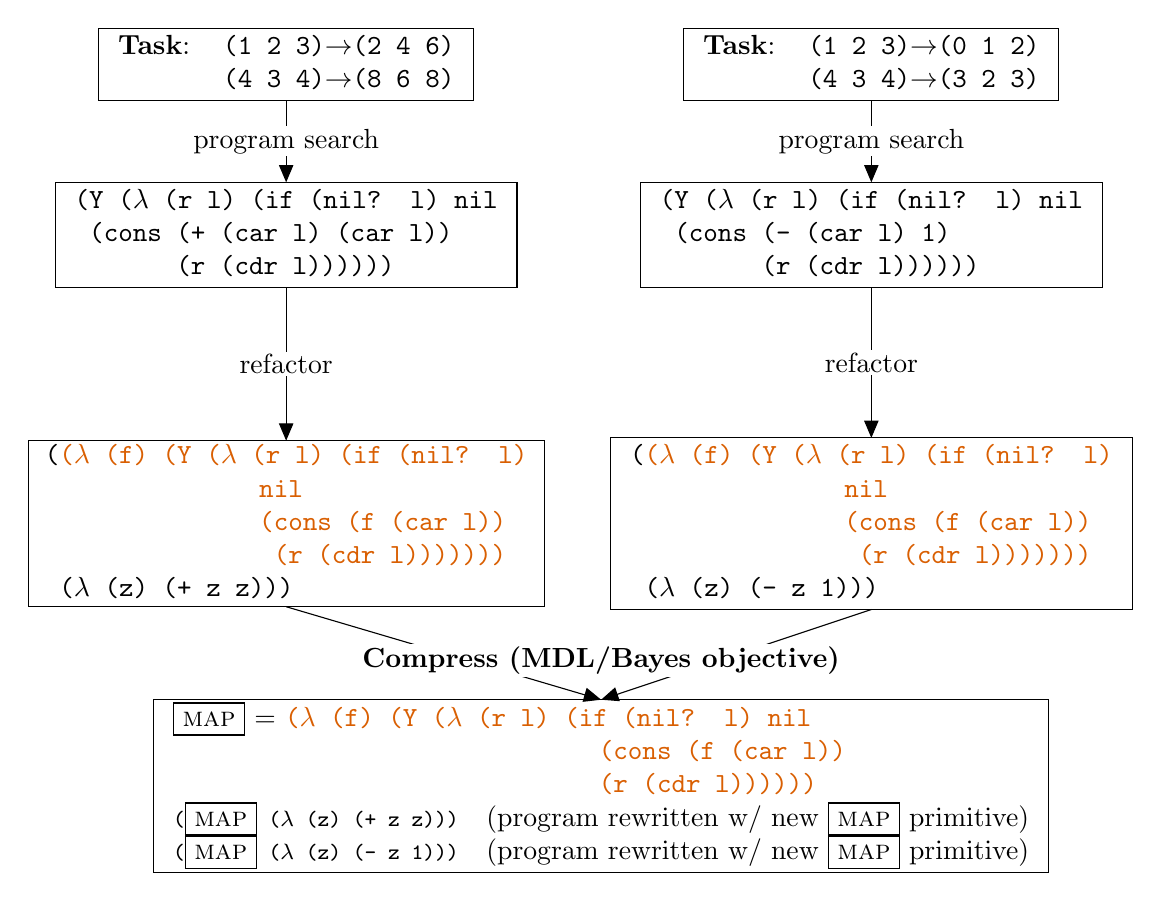
\begin{tikzpicture}[every node/.style={inner sep=1,outer sep=0}]
    \node(p1)[draw] at (-1,0) {
      \begin{tabular}{l}
      \texttt{(Y ($\lambda$ (r l) (if (nil? l) nil}\\
      \texttt{ (cons (+ (car l) (car l))}\\
      \phantom{\texttt{(cons }}\texttt{ (r (cdr l))))))}
    \end{tabular}
    };
    \node(r1)[draw,inner sep=0,outer sep=0] at ([yshift=-3cm]p1.south) {
      \begin{tabular}{l}
  \texttt{(}\orange{\texttt{($\lambda$ (f) (Y ($\lambda$ (r l) (if (nil? l)}}\\
\phantom{(($\lambda$ (f) (Y ($\lambda$ (r l)}\orange{\texttt{nil}}\\
\phantom{(($\lambda$ (f) (Y ($\lambda$ (r l)}\orange{\texttt{(cons (f (car l))}}\\
\phantom{(($\lambda$ (f) (Y ($\lambda$ (r l)}\orange{\texttt{ (r (cdr l)))))))}}\\
\texttt{ ($\lambda$ (z) (+ z z)))}
      \end{tabular}
    };

        \node(p2)[draw] at ([xshift=4.5cm]p1.east) {
    \begin{tabular}{l}
      \texttt{(Y ($\lambda$ (r l) (if (nil? l) nil}\\
      \texttt{ (cons (- (car l) 1)}\\
      \phantom{\texttt{(cons }}\texttt{ (r (cdr l))))))}
    \end{tabular}
    
    };
    \node(r2)[draw] at ([yshift=-3cm]p2.south) {
\begin{tabular}{l}
  \texttt{(}\orange{\texttt{($\lambda$ (f) (Y ($\lambda$ (r l) (if (nil? l)}}\\
\phantom{(($\lambda$ (f) (Y ($\lambda$ (r l)}\orange{\texttt{nil}}\\
\phantom{(($\lambda$ (f) (Y ($\lambda$ (r l)}\orange{\texttt{(cons (f (car l))}}\\
\phantom{(($\lambda$ (f) (Y ($\lambda$ (r l)}\orange{\texttt{ (r (cdr l)))))))}}\\
\texttt{ ($\lambda$ (z) (- z 1)))}
      \end{tabular}

    };

    \draw [->] (p1.south)  --(r1.north) node[fill=white,midway] {refactor};
    \draw [->] (p2.south)  --(r2.north) node[fill=white,midway] {refactor};

    \node[draw](m) at (3,-7) {
\begin{tabular}{l}
          \fbox{\textsc{map}} = \orange{\texttt{($\lambda$ (f) (Y ($\lambda$ (r l) (if (nil? l) nil}}\\
  \phantom{\texttt{\emph{map}} = \texttt{($\lambda$ (f) (Y ($\lambda$ (r l) (if }}\orange{\texttt{(cons (f (car l))}}\\
  \phantom{\texttt{\emph{map}} = \texttt{($\lambda$ (f) (Y ($\lambda$ (r l) (if }}\orange{\texttt{(r (cdr l))))))}}\\
  \code{(}\fbox{\textsc{map}}\code{ ($\lambda$ (z) (+ z z)))}\quad(program rewritten w/ new \fbox{\textsc{map}} primitive)\\
  \code{(}\fbox{\textsc{map}}\code{ ($\lambda$ (z) (- z 1)))}\quad(program rewritten w/ new \fbox{\textsc{map}} primitive)\\
      \end{tabular}      
    };
    \draw [->](r1.south)--(m.north);
    \draw [->](r2.south)--(m.north);
    \node[fill=white] at ([yshift=0.5cm]m.north) {\textbf{Compress (MDL/Bayes objective)}};
    %% \visible<2-3>{
    %%   \node[fill=orange!50!white,align=center] at (r1) {\Huge $10^{14}$\\\Huge  refactorings };
    %%   \node[fill=orange!50!white,align=center] at (r2) {\Huge $10^{13}$\\\Huge  refactorings };
    %% }
    %% \visible<3>{
    %%   \node[fill=orange!50!white,align=center] at ([yshift=7cm]m.north) {\Huge version space: set of programs\\
    %%   \huge Lau 2003; Gulwani 2012};
    %%   }
    %% \visible<4>{
    %%   \node[fill=orange!50!white,align=center] at (r1) {\Huge $\leq 10^6$\\\Huge version spaces };
    %%   \node[fill=orange!50!white,align=center] at (r2) {\Huge $\leq 10^6$\\\Huge version spaces };
    %% }

       \node(t1)[draw] at ([yshift=1.5cm]p1.north) {\begin{tabular}{ll}
           \textbf{Task}:&\texttt{(1 2 3)$\to$(2 4 6)}\\
           &\texttt{(4 3 4)$\to$(8 6 8)}
       \end{tabular}};
       \draw [->] (t1.south)  --(p1.north) node[fill=white,midway] {program search};
       \node(t2)[draw] at ([yshift=1.5cm]p2.north) {\begin{tabular}{ll}
           \textbf{Task}:&\texttt{(1 2 3)$\to$(0 1 2)}\\
           &\texttt{(4 3 4)$\to$(3 2 3)}
       \end{tabular}};
       \draw [->] (t2.south)  --(p2.north) node[fill=white,midway] {program search};
       
  \end{tikzpicture}
  \caption{DSL learning as code refactoring. For each task we discover programs during waking, then refactor the code from those programs to expose common subprograms (highlighted in \orange{orange}). Common subprograms are incorporated into the DSL when they increase a Bayesian objective. Intuitively, these new DSL components best compress the programs found during waking.}\label{mapFactor}
  \end{figure*}

\begin{comment}

We propose these new expressions
by extracting fragments of programs already in the frontiers
(Tbl.~\ref{fragmentExample}).  An important point here is that we are
\emph{not} simply adding subexpressions of programs to $\mathcal{D}$,
as done in the EC algorithm~\cite{Dechter:2013:BLV:2540128.2540316}
and other prior work~\cite{DBLP:conf/ecai/LinDETM14}.  Instead, we are
extracting fragments that unify with programs in the frontiers.  This
idea of storing and reusing fragments of expressions comes from
Fragment Grammars~\cite{tim} and Tree-Substitution
Grammars~\cite{cohn2010inducing}, and is closely related to the idea
of antiunification~\cite{henderson2013cumulative}.

%\vfill\null

%\columnbreak



To define the prior distribution over $(\mathcal{D},\theta})$, we penalize the syntactic complexity of the $\lambda$-calculus expressions in the DSL, defining $    \probability[\mathcal{D}]\propto\exp(-\lambda\sum_{p\in \mathcal{D}}\text{size}(p) )$ where $\text{size}(p)$  measures the size of the syntax tree of program $p$,
  and $\lambda$ controls how strongly we regularize the size of the DSL.
  We place a symmetric Dirichlet prior over the weight vector $\theta$,
  defining 
$  \probability[\theta|\mathcal{D}] = \text{Dir}(\theta|\alpha)$, where
 $\alpha$ is a concentration parameter controlling the smoothness of the prior over $\theta$.
%Alg.~\ref{grammarInductionAlgorithm} specifies the DSL induction algorithm.

To appropriately score each proposed $\mathcal{D}$ we must reestimate
 the weight vector $\theta$.
Although this  may seem 
very similar to estimating the parameters of a probabilistic context free grammar,
for which we have effective approaches like the Inside/Outside algorithm~\cite{international2000derivation},
our DSLs are context-sensitive due to the presence of variables
in the programs and also due to the polymorphic typing system.
In the Supplement we derive a tractable MAP estimator for $\theta$.
%% Putting all these ingredients together, Alg.~\ref{mainAlgorithm} describes how we combine program search,
%% recognition model training, and DSL induction.

\begin{figure*}[!htb]\tabcolsep=2pt
\centering  \begin{minipage}[c]{0.2\textwidth}
  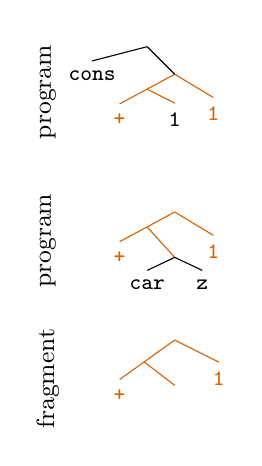
\begin{tikzpicture}[scale=0.7]
    %% \node[rotate=30] at (-2,0) {\begin{tabular}{c}
    %%     \footnotesize Program:\\
    %%     \code{($\lambda$ (x) (+ (- x) 1))}
    %% \end{tabular}};
    %\node at (,0.5) {\code{cons}};
    \node [rotate=90] at (-2.3,-0.5) {\small program};
    
          \node(l1) at (0,0) {};
  \node[color=pop3](p1) at (-1,-1) {\code{+}};
  \node[color=pop3](n1) at (0.7,-0.9) {\code{1}};
  \node(x1) at (0,-1) {\code{1}};
  \draw[color=pop3] (l1.south) -- (p1.north);
  \draw[color=pop3] (l1.south) -- (n1.north);
  \draw[color=pop3] (-0.5,-0.45) -- (x1.north);

  \node(t) at (-0.5,0.5) {};
  \draw (l1.south) -- (t.south);
  \node(c) at (-1.5,-0.2) {\code{cons}};
  \draw (t.south) -- (c.north);
  
%    \draw  (l1.south) -- (-0.5,0.5);

  %% \node(c) at (-0.5,-1.5) {\code{-}};
  %% \node(z) at (0.5,-1.5) {\code{x}};

  %% \draw (0,-1) -- (c.north);
  %% \draw (0,-1) -- (z.north);
  
  \begin{scope}[shift={(0,-2.5)}]
      \node(l1) at (0,0) {};
  \node[color=pop3](p1) at (-1,-1) {\code{+}};
  \node[color=pop3](n1) at (0.7,-0.9) {\code{1}};
  %\node(x1) at (0,-1) {};
  \draw[color=pop3] (l1.south) -- (p1.north);
  \draw[color=pop3] (l1.south) -- (n1.north);
  \draw[color=pop3] (-0.5,-0.45) -- (0,-1);


  \node(c) at (-0.5,-1.5) {\code{car}};
  \node(z) at (0.5,-1.5) {\code{z}};

  \draw (0,-1) -- (c.north);
  \draw (0,-1) -- (z.north);

  \node [rotate=90] at (-2.3,-0.7) {\small program};
  
  \end{scope}

\begin{scope}[shift={(0,-5)}]
  \node[pop3](p1) at (-1,-1) {\code{+}};
  \node[pop3](n1) at (0.8,-0.7) {\code{1}};
  \node[pop3](a) at (0,-1) {\code{ }};
  %\node(x1) at (0,-1) {};
  \draw[pop3] (0,0) -- (p1.north);
  \draw[pop3] (0,0) -- (n1.north);
  \draw[pop3] (-0.55,-0.4) -- (a.north);
  \node [rotate=90] at (-2.3,-0.7) {\small fragment};

  \end{scope}

\end{tikzpicture}
  \end{minipage}
\hspace{0.1cm}\begin{tabular}{ll}
    \toprule
    Example programs in frontiers&Proposed $\lambda$-expression\\\midrule
    \begin{tabular}{l}
      \code{($\lambda$ ($\ell$) (map ($\lambda$ (x) (index x $\ell$))}\\
      \phantom{\code{($\lambda$ ($\ell$) (map }}\code{(range (- (length $\ell$) 1))))}\\
      \code{($\lambda$ ($\ell$) (map ($\lambda$ (x) (index x $\ell$))}\\
      \phantom{\code{($\lambda$ ($\ell$) (map }}\code{(range (+ 1 1))))}\\
    \end{tabular}&
    \begin{tabular}{l}
      \code{(map ($\lambda$ (x) (index x $\ell$))}\\
      \phantom{\code{(map)}}\code{(range $\alpha$))}\\
    \end{tabular}\\\midrule
    \begin{tabular}{l}
      \code{($\lambda$ (s) (map ($\lambda$ (x)}\\
      \hspace{0.4cm}\code{ (if (= x '.') '-' x))) s)}\\
      \code{($\lambda$ (s) (map ($\lambda$ (x) }\\
      \hspace{0.4cm}\code{ (if (= x '-') ',' x))) s)}\\
      \end{tabular}&
    \begin{tabular}{l}      \code{($\lambda$ (s) (map ($\lambda$ (x)}\\\hspace{0.2cm}\code{   (if (= x $\alpha$) $\beta$ x))) s)}
      \end{tabular}
\\\bottomrule\\
\end{tabular}
\caption{\textbf{Left:} syntax trees of two programs sharing common structure,
highlighted in {\orange{orange}},
  from which we extract a fragment and add it to the DSL (bottom). \textbf{Right:} actual programs,
  from which we extract fragments that  (top) slice from the beginning of a list or (bottom) perform character substitutions.}\label{fragmentExample}
\end{figure*}

  \end{comment}
\begin{comment}
  \begin{wrapfigure}{R}{0.6\textwidth}
  \begin{minipage}{0.6\textwidth}    
    \begin{algorithm}[H]
      \caption{The \system Algorithm}
      \label{mainAlgorithm}
      \begin{algorithmic}
        \STATE {\bfseries Input:} Initial DSL $\mathcal{D}$, set of tasks $X$, iterations $I$
        \STATE \textbf{Hyperparameters:} Enumeration timeout $T$
        %     \STATE \textbf{Output:} DSL $\mathcal{D}$, weight vector $\theta$, recognition model $q(\cdot)$
        \STATE Initialize $\theta\gets \text{uniform}$ %, $q_0(\cdot ) = \theta_0$
        \FOR{$i=1$ {\bfseries to} $I$}
        %     \FOR{$x:\tau\in X$}
        \STATE  $\mathcal{F}^{\theta}_x\gets \{p| p\in
        \text{enum}(\mathcal{D},\theta,T)\text{ if }\probability[x|p] > 0\}$
        \footnotesize{\hspace{0.1cm}(\textbf{Search})}
        \STATE $q\gets \text{train recognition model, maximizing }\mathcal{L}_{\text{RM}}$ \hspace{0.2cm}(\footnotesize{\textbf{Compile}})
        \STATE  $\mathcal{F}^{q}_x\gets\{p|p\in
        \text{enum}(\mathcal{D},q(x),T)\text{ if }\probability[x|p] > 0\}$
        \footnotesize{\hspace{0.15cm}\textbf{(Search)}}
        
        \STATE $\mathcal{D},\theta\gets $induceDSL$(\{\mathcal{F}^{\theta}_x\cup\mathcal{F}^{q}_x\}_{x\in X})$  \hspace{1.1cm} \footnotesize{\textbf{(Compress)}}
        %% \STATE Define $Q_x(z) \propto \begin{cases}
        %%   \probability[x|z]\probability[z|\mathcal{D}_i,\theta_i]&x\in \mathcal{F}_x\\
        %%   0&x\not \in \mathcal{F}_x
        %% \end{cases}
        \ENDFOR
        \STATE \textbf{return} $\mathcal{D},\theta,q$
      \end{algorithmic}
    \end{algorithm}
  \end{minipage}
\end{wrapfigure}
  \end{comment}

\section{Experiments}

\subsection{Programs that manipulate sequences}\label{sequences}
We apply \system to list processing %% (Section~\ref{listSection})
and text editing, %% (Section~\ref{textSection})
using a GRU~\cite{cho2014learning} for
the recognition model, and initially providing the system with generic sequence manipulation primitives:
\code{foldr}, \code{unfold}, \code{if}, \code{map}, \code{length},
\code{index}, \code{=}, \code{+}, \code{-}, \code{0}, \code{1}, \code{cons},
\code{car}, \code{cdr}, \code{nil}, and \code{is-nil}.



%\subsubsection{List Processing}\label{listSection}
\textbf{List Processing:} Synthesizing programs that manipulate data structures is a widely studied
problem in the programming languages community~\cite{feser2015synthesizing}.
%with applications to computer aided programming~\cite{solar2008program}.
We consider this problem within the context of learning functions that
manipulate lists, and also perform arithmetic operations upon lists (Table~\ref{listExamples}).
We created 236 human-interpretable list manipulation tasks, each with 15
input/output examples.
%% Our data set is interesting in three major ways: many of the tasks
%% require complex solutions; the tasks were not generated from some
%% latent DSL, and the agent must learn to solve these complicated
%% problems from only 236 tasks.
%% Our data set assumes arithmetic operations as well as sequence operations,
%% so we additionally provide our system with the following arithmetic
%% primitives: \code{mod}, \code{*}, \code{>}, \code{is-square},
%% \code{is-prime}.
%% evaluating  on a 50/50 test/train split.
In solving these tasks, the system
composed 38 new subroutines, and rediscovered the higher-order
function \code{filter} ($f_1$ in Table~\ref{initialExampleDSL}, left).%% , yielding a more expressive DSL more closely
%% matching the domain (Tbl.~\ref{initialExampleDSL}, left).
\begin{figure}[b]\centering
\vspace{-0.5cm}  \begin{tabular}{lll}
    \toprule
    Name & Input & Output \\\midrule
    repeat-3 & [7\, 0] & [7\, 0\, 7\, 0\, 7\, 0] \\
    drop-3 & [0\, 3\, 8\, 6\, 4] & [6\, 4] \\
    rotate-2 & [8\, 14\, 1\, 9] & [1\, 9\, 8\, 14] \\
    count-head-in-tail & [1\, 2\, 1\, 1\, 3] & 2 \\
    keep-div-5 & [5\, 9\, 14\, 6\, 3\, 0] & [5\, 0] \\
    product & [7\, 1\, 6\, 2] & 84 \\
    \bottomrule
  \end{tabular}
  \captionof{table}{Some tasks in our list function domain.}\label{listExamples}\vspace{-0.5cm}
\end{figure}

%\subsubsection{Text Editing}\label{textSection}
\textbf{Text Editing:} Synthesizing programs that edit text is a classic problem in the
programming languages and AI literatures~\cite{gulwani2011automating,lau2001programming}.
This prior work uses hand-engineered DSLs.
Here, we instead start out with generic sequence manipulation
primitives and recover many of the higher-level building blocks that 
have made these other systems successful.
%% Because our enumerative search procedure cannot generate string %
%% constants, we instead enumerate programs with string-valued
%% parameters.  For example, to learn a program that prepends ``Dr.'', we
%% enumerate $\text{\code{(}}f_3\code{ string s)}$ -- where $f_3$ is the
%% learned appending primitive (Fig.~\ref{initialExampleDSL}) --- and then
%% define $\probability[x|p]$ by approximately marginalizing out the
%% string parameters via a simple dynamic program.
%% In Sec.~\ref{regressionSection}, we will use a similar trick to
%% synthesize programs containing real numbers, but using gradient
%% descent instead of dynamic programming.

We trained our system on 109 automatically-generated text editing tasks, with 4 input/output examples each.
After three iterations, it assembles a DSL containing a dozen new functions (Fig.~\ref{initialExampleDSL}, center) solving
all the training tasks.
But, how well does the  learned DSL generalized to real text-editing scenarios?
We tested, but did not train, on the 108 text editing problems from the SyGuS~\cite{alur2016sygus} program synthesis competition. Before any learning,
\system solves 3.7\% of the problems with an average search time of 235 seconds.
After learning,
it solves 74.1\%, and does so much faster,
solving them in an average of 29 seconds.
As of the 2017 SyGuS competition,
the best-performing algorithm solves 79.6\% of the problems.
But, SyGuS comes with a
different hand-engineered DSL \emph{for each text editing problem}. %\footnote{SyGuS text editing problems also prespecify the set of allowed string constants for each task. For these experiments, our system did not use this assistance.}
Here  we learned a single DSL
that applied generically to
all of the tasks,
and perform comparably to the best
prior work.

\subsection{Symbolic Regression: Programs from visual input}\label{regressionSection}
We apply \system
to symbolic regression problems.  Here, the
agent observes points along the curve of a function, and must write a
program that fits those points.  We initially equip our learner with
addition, multiplication, and division, and task it with solving
100 %% symbolic regression
problems, each either a polynomial or rational function.  The recognition model is a
convnet that observes an image of the target function's
graph (Fig.~\ref{functions}) --- visually, different kinds of
polynomials and rational functions produce different kinds of graphs,
and so the convnet can  look at a graph and predict
what kind of function best explains it.
A key difficulty, however, is
that these problems are best solved with programs containing real
numbers.  Our solution to this difficulty is to enumerate
 programs with real-valued parameters, and then fit those
parameters by automatically differentiating through the programs the
system writes and use gradient descent to fit the parameters.
We define the likelihood model, $\probability[x|p]$, by assuming a Gaussian noise model for the input/output examples,
and penalize the use of real-valued parameters using the BIC~\cite{Bishop:2006:PRM:1162264}.
\begin{figure}\vspace{-0.0cm} \newcommand{\functionSize}{1.1cm}\centering
  \begin{minipage}[c]{0.3\columnwidth}%\vspace{-0.3cm}
  
\includegraphics[width = \functionSize]{figures/functions/6.png}
  
\includegraphics[width = \functionSize]{figures/functions/48.png}\\
  
\includegraphics[width = \functionSize]{figures/functions/102.png}
  
\includegraphics[width = \functionSize]{figures/functions/116.png}\\
  \vspace{1pt}%
\includegraphics[width = \functionSize]{figures/functions/181.png}
  %
\includegraphics[width = \functionSize]{figures/functions/160.png}
  
\includegraphics[width = \functionSize]{figures/functions/160.png}
    
\includegraphics[width = \functionSize]{figures/functions/149.png}
  \end{minipage}
  \begin{minipage}[c]{0.69\columnwidth}    
    \caption{Recognition model input for symbolic regression. DSL learns subroutines for polynomials (top rows) and rational functions (bottom) while the recognition  model jointly learns to look at a graph of the function (left) and predict which learned subroutines best explain the observation.}\label{functions}\vspace{-1cm}
        \end{minipage}
\end{figure}
We learn a DSL containing 13 new functions,
mainly templates for polynomials of different orders or ratios of polynomials.
The model also learns to find programs minimizing the number of continuous parameters ---
learning to represent linear functions with 
\code{(* real (+ x real))}, which has two continuous parameters, and represents quartic functions using $f_4$ in the rightmost column of Fig.~\ref{initialExampleDSL}
which has five continuous parameters.
This phenomenon arises from our Bayesian framing:
both the generative model's bias toward shorter programs,
and the likelihood model's BIC penalty.

\subsection{Learning from Scratch}
A long-standing dream within the program induction community
is ``learning from scratch'': starting with a \emph{minimal} Turing-complete programming language,
and then learning to solve a wide swath of
induction problems~\cite{solomonoff1964formal,schmidhuber2004optimal,hutter2004universal,solomonoff1989system}.
All existing systems,
including ours,
fall far short of this dream,
and it is unclear (and we believe unlikely)
that this dream could ever be fully realized.
How far can we push in this direction?
``Learning from scratch'' is subjective, but a reasonable
starting point is the set of primitives provided in 1959
Lisp~\cite{mccarthy1960recursive}: these include
conditionals, recursion, arithmetic, and the 
list operators \code{cons}, \code{car}, \code{cdr}, and \code{nil}.
A  basic first goal is to start with
these primitives,
and then recover a DSL that
more closely resembles modern functional languages like Haskell and OCaml.
Recall (Sec.~\ref{sequences})
that we initially provided our system with functional programming routines like
\code{map} and \code{fold}.

We ran the following experiment: \system was given a subset of
the 1959 Lisp primitives, and tasked with solving 22
programming exercises. A key difference between
this setup and our previous experiments is that,
for this experiment,
the system is
given primitive recursion,
whereas previously we had sequestered recursion within
higher-order functions like \code{map}, \code{fold}, and \code{unfold}.

After running for 93 hours on 64 CPUs, our
algorithm solves these 22 exercises, along the way assembling a DSL
with a modern repertoire of
functional programming idioms and subroutines, including \code{map},
\code{fold}, \code{zip}, \code{unfold}, \code{index}, \code{length},
and  arithmetic operations like 
building lists of natural numbers between an interval (see Figure~\ref{learningFromScratch}).
We did not use the recognition model for this experiment:
a bottom-up pattern recognizer is of little use
for acquiring this abstract knowledge
from less than two dozen problems.

\begin{figure*}  \newcommand{\helpSize}{0.25cm}
  \begin{tabular}{cc}\toprule
    \normalsize \pop{Programs} \& Tasks&\normalsize \popp{DSL}\\\midrule 
    

    %\rotatebox[origin=c]{90}{\normalsize \pop{Programs} \& Tasks}&
    \begin{tabular}{l}
\code{[2\, 1\, 4]$\to$[2\, 1\, 4\, 0]}\\
%\code{[9\, 4\, 8]$\to$[9\, 4\, 8\, 0]}\\
\code{[9\, 8]$\to$[9\, 8\, 0]}\\
\blueCode{$f(\ell) = $($f_2$ cons $\ell$ (cons 0 nil))}\\\\

\code{[2\, 5\, 6\, 0\, 6]$\to$19}\\
\code{[9\, 2\, 7\, 6\, 3]$\to$27}\\
\blueCode{$f(\ell) = $($f_2$ + $\ell$ 0)}\\\\

\code{[4\, 2\, 6\, 4]$\to$[8\, 4\, 12\, 8]}\\
%\code{[0\, 3\, 5\, 0\, 3\, 2]$\to$[0\, 6\, 10\, 0\, 6\, 4]}\\
\code{[2\, 3\, 0\, 7]$\to$[4\, 6\, 0\, 14]}\\
\blueCode{$f(\ell) = $($f_3$ ($\lambda$ (x) (+ x x)) $\ell$)}\\\\


      \code{[1\, 5\, 2\, 9]}$\to$\code{[1\, 2]}\\
      \code{[3\, 8\, 1\, 3\, 1\, 2]}$\to$\code{[3\, 1\, 1]}\\
      \blueCode{$f(\ell) = $($f_0$ empty? car}\\
      \phantom{\blueCode{$f(\ell) = $($f_0$}}\blueCode{($\lambda$ (l) (cdr (cdr l))) $\ell$)}
      \\
      
      \end{tabular}&

%    \rotatebox[origin=c]{90}{\normalsize \popp{DSL}}&
    \begin{tabular}{l}
        \popp{\code{$f_0($p$,$f$,$n$,$x$)\,=\,$(if (p x) nil}}\\
      \phantom{\code{$f_1($f$,$l$,$x$)\,=\,$(if }}}\popp{\code{(cons (f x) ($f_0$ (n x))))}}\\
        \hspace{\helpSize}($f_0$: \emph{unfold})\\
        \popp{\code{$f_1($i$,$l$)\,=\,$(if (= i 0) (car l)}}\\
      \phantom{\code{$f_1($f$,$l$,$x$)\,=\,$(if}}}\popp{\code{($f_1$ (- i 1) (cdr l))))}}\\
        \hspace{\helpSize}($f_1$: \emph{index})\\
        \popp{\code{$f_2($f$,$l$,$x$)\,=\,$(if (empty? l) x}}\\
      \phantom{\code{$f_2($f$,$l$,$x$)\,=\,$(if }}}\popp{\code{(f (car l) ($f_2$ (cdr l))))}}\\
        \hspace{\helpSize}($f_2$: \emph{fold})\\
        \greenCode{$f_3($f$,$l$)\,=\,$($f_2$ nil l ($\lambda$ (x a) (cons (f x) a)))}\\
        \hspace{\helpSize}($f_3$: \emph{map})\\
        \greenCode{$f_4(\ell)$\,=\,(if (empty? $\ell$) 0 (+ 1 ($f_4$ (cdr $\ell$)))))}\\
        \hspace{\helpSize}($f_4$: \emph{length})\\
        \greenCode{$f_5(n)$\,=\,($f_0$ (= $n$) ($\lambda$ (x) x) (+ 1) 0)}\\
        \hspace{\helpSize}($f_5$: \emph{range})

%        -0.222777	int -> int -> list(int)	#(lambda (lambda (fix1 $0 (lambda (lambda (#(lambda (lambda (lambda (if $0 empty (cons $1 $2))))) (map (lambda (#(+ 1) $0)) ($1 (#(lambda (- $0 1)) $0))) 0 (eq? $0 $3)))))))

      \end{tabular}
    %% : (lambda (#(#(lambda (lambda (lambda (lambda (fix1 $0 (lambda (lambda (if (empty? $0) $3 ($4 ($5 $0) ($1 (cdr $0))))))))))) (lambda (car $0))) (lambda (lambda (+ $0 $1))) 0 $0))
    %% (lambda (lambda (lambda (lambda (fix1 $0 (lambda (lambda (#(lambda (lambda (lambda (if $0 empty (cons $1 $2))))) ($1 ($3 $0)) ($4 $0) ($5 $0)))))))))
    %% (lambda (lambda (fix1 $0 (lambda (lambda (#(lambda (lambda (lambda (if $0 empty (cons $1 $2))))) (#(lambda (lambda (fix1 $0 (lambda (lambda (if (empty? $0) empty (cons ($3 (car $0)) ($1 (cdr $0))))))))) (lambda (#(+ 1) $0)) ($1 (#(lambda (- $0 1)) $0))) 0 (eq? $0 $3)))))))
    \\\bottomrule 
    \end{tabular}
  \caption{Bootstrapping a standard library of functional programming routines, starting from recursion along with primitive operations found in 1959 Lisp.}\label{learningFromScratch}
  \end{figure*} 

We believe that program learners should \emph{not}
start from scratch,
but instead should start from
a rich, domain-agnostic
basis like those embodied in the standard libraries of modern  languages.
What this experiment shows is that \system doesn't \emph{need} to start from a rich basis,
and can in principle recover many of the amenities of modern programming systems,
provided it is given enough computational power and a suitable
spectrum of tasks.% programming exercises.

\subsection{Learning Generative Models}

We apply \system to learning generative models for images and text (Fig.~\ref{geomCompiled}-\ref{regularExpressions}).
For images, we learn programs controlling a simulated ``pen,''
and the task is to look at an image and explain it in terms of a graphics program.
For text, we learn probabilistic regular expressions -- a simple probabilistic program for which inference is always tractable -- and the task is to
infer a regex from a collection of strings.
\begin{figure}[t]
  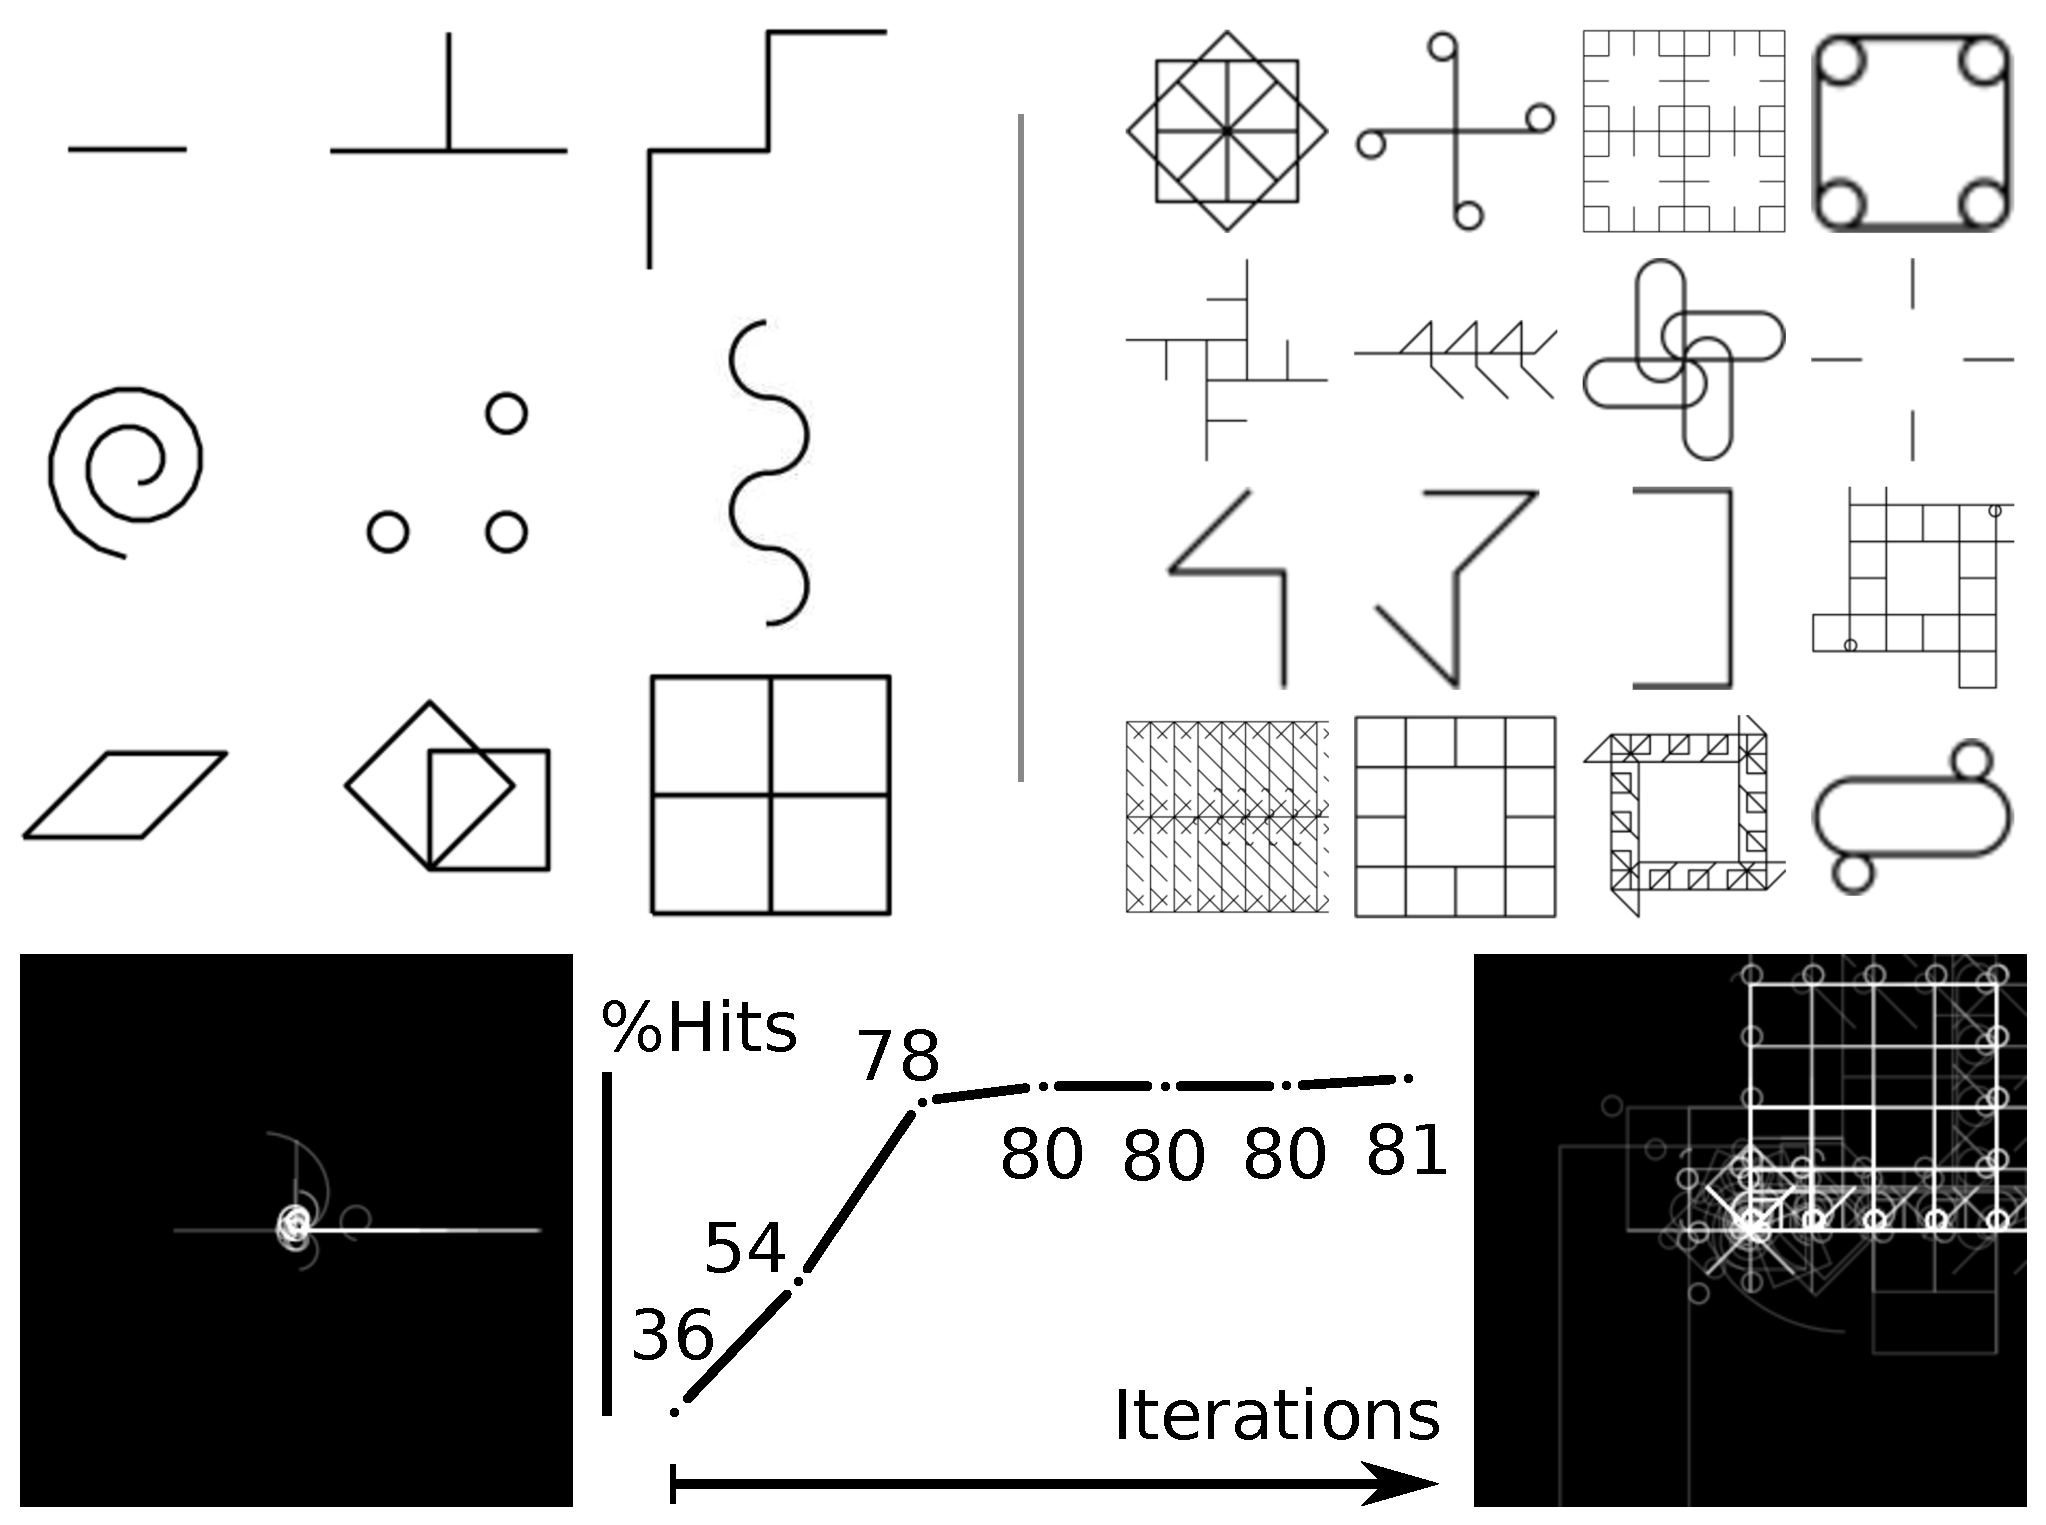
\includegraphics[width=\columnwidth]{figures/geomCompiled.eps} 
  \caption{
  Top left: Example training tasks. Top right: samples from the learned DSL.
 Bottom: \% holdout testing tasks solved (middle); on the sides are averaged samples from the DSL
  before any training (left) and after last iteration (right).}\label{geomCompiled}

  \end{figure}

\begin{figure}
\centering
\tiny
\tabcolsep=2pt
\vspace{0pt}
\begin{tabular}{cc}
\begin{tabular}{ccc}
\multicolumn{3}{c}{Tasks:}\\
\hline
1.14531&F&110.9 \\ 
?&CL&163.2 \\
1.29857&F&207.3\\
?&PCFL&143.3 \\
\multicolumn{3}{c}{Learned generative models:}\\
\hline
 \scode{\textbackslash?\textbar(1\textbackslash .\textbackslash d+)}& \scode{((\textbackslash u\textbackslash u)*)\textbar F}& \scode{\textbackslash d\textbackslash d\textbackslash d\textbackslash.\textbackslash d} \\
 \multicolumn{3}{c}{Samples from synthesized generative models:}\\
\hline
1.61&DQDF& 343.8 \\ 
?&F&241.2\\
?&F&647.5\\
1.2&KI&246.8\\
1.5080987&F&728.6\\
?&GL&029.3\\
1.453&F&289.1\\
    \hline
        \\
\end{tabular} 
&
\begin{tabular}{c}
\begin{tabular}{l}
\multicolumn{1}{c}{Learned DSL:}\\
\hline
$f_1() = $ \scode{\textbackslash u\textbackslash w*}\\
$f_2(x) = $ \scode{($x$|$f_1$)*} $=$ \scode{($x$|\textbackslash u\textbackslash w*)*}\\
$f_3(x) =  f_2(\scode{space}) = $\scode{( \textbar\textbackslash u\textbackslash w*)*}\\
\hline
$f_4(x) = $ \scode{($x$*$x$)}\\
\emph{ (equivalent to regex `plus')}\\
$f_5() = f_4(\scode{\textbackslash l}) = \scode{\textbackslash l*\textbackslash l}$\\
    \hline
\end{tabular}
\\
\\
\includegraphics[width=.4\linewidth]{figures/nampiregexjoshcurve3.eps} 
\end{tabular}
\end{tabular}
\vspace{-.3cm}
\caption{regex stuff}
\end{figure}


\subsection{Quantitative Results on Held-Out Tasks}\label{quantitative}
We evaluate  on held-out testing tasks,
measuring how many
tasks are solved and how long it takes to solve them (Fig.~\ref{learningCurves}).
Prior to any learning,
the system cannot find solutions for most of the tasks,
and those it does solve take a long time;
with more wake/sleep iterations,
we converge upon DSLs and recognition models 
more closely matching the domain.

%% We compare with ablations of our model on held out tasks.
%% The purpose of this ablation study is 
%% both to examine the role of each component of \systemEnding,
%% as well as to compare with
%% prior approaches in the literature:
%% a head-to-head
%% comparison of program synthesizers is complicated by the fact that
%% each system, including ours, makes idiosyncratic 
%% assumptions about the space of programs and the statement of tasks.

%% Nevertheless, much prior work can be modeled within our setup. 
%% We compare with the following ablations (Tbl~\ref{baselineComparisons};
%% Fig~\ref{learningCurves}):
%% \\\noindent \textbf{No NN:} lesions the recognition model.
%% \\\noindent \textbf{NPS}, which does not learn the DSL,
%% instead learning the recognition model
%% from samples drawn from the fixed DSL.
%% We call this NPS (Neural Program Synthesis)
%% because this is closest to how
%% RobustFill~\cite{devlin2017robustfill} and DeepCoder~\cite{balog2016deepcoder} are trained.
%% \\\noindent \textbf{SE}, which lesions the recognition model and restricts the DSL  learning algorithm to
%% only add \textbf{S}ub\textbf{E}xpressions of programs in the frontiers to the DSL. This is how most prior approaches have learned libraries of functions~\cite{Dechter:2013:BLV:2540128.2540316,DBLP:conf/icml/LiangJK10,DBLP:conf/ecai/LinDETM14}.
%% \\\noindent \textbf{PCFG}, which lesions the recognition model and does not learn the DSL,
%% but instead learns the parameters of the DSL ($\theta$), learning the parameters of a PCFG while not learning any of the structure.
%% \\\noindent \textbf{Enum}, which enumerates a frontier without any learning --- equivalently, our first search step.
%For each domain,
%% We are interested both in how many tasks the
%% agent can solve and how quickly it can find those solutions.
%% Tbl.~\ref{baselineComparisons}
%% compares our model against these alternatives.
%% We consistently
%% improve on the baselines,
%% and find that lesioning the recognition model
%% and lesioning it also slows down the convergence of the algorithm,
%% taking more iterations to reach a given number of tasks solved (Fig.~\ref{learningCurves}).
%% This supports a view of the recognition model as a way of amortizing the cost of search.



\begin{figure*}\centering
  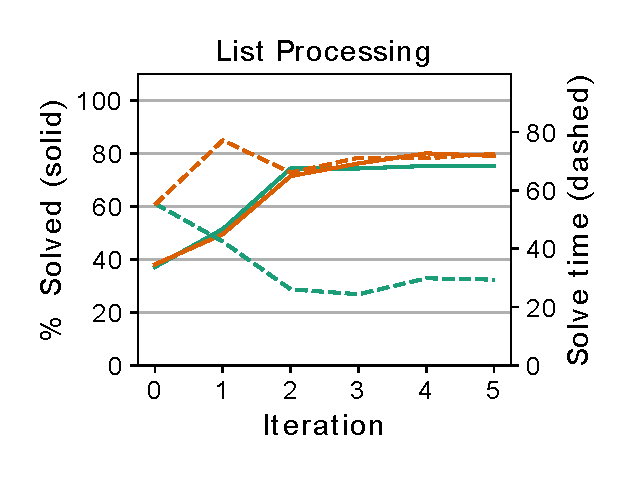
\includegraphics[width = 4.5cm]{figures/listLearningCurve.eps} \qquad
  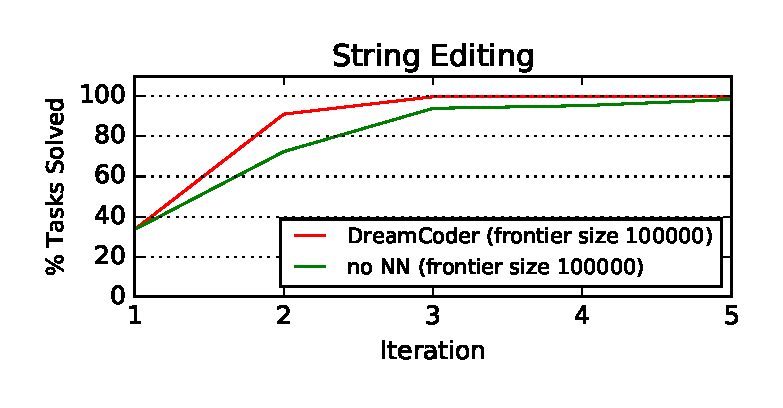
\includegraphics[width = 4.5cm]{figures/textLearningCurve.eps}\qquad
  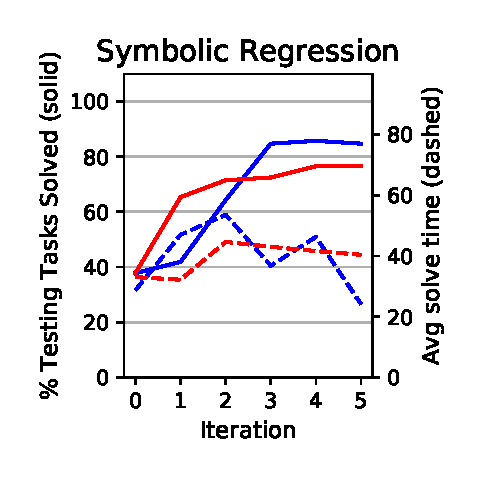
\includegraphics[width = 4.5cm]{figures/rationalCurve.eps}
\vspace{-0.4cm}  \caption{Learning curves for \system both with (\orange{in orange}) and without
    (\teal{in teal}) the recognition model. Solid lines: \% holdout testing tasks solved w/ 10m timeout. Dashed lines: Average solve time, averaged only over tasks that are solved.}\label{learningCurves}\vspace{-0.5cm}
\end{figure*}

\section{Discussion}



%\paragraph{Outlook.}
We contribute an algorithm, \systemEnding, that learns to program by
bootstrapping a DSL with new domain-specific primitives that the algorithm
itself discovers, together with a neural recognition model that learns to
efficiently deploy the DSL on new tasks. %% We believe this integration of top-down
%% symbolic representations and bottom-up neural nets --- both of them learned
%% --- can help make program induction systems more generally useful for AI. 
%Many
%directions remain open.
%\paragraph{Future.}
Two immediate future goals are to integrate more sophisticated neural recognition
models~\cite{devlin2017robustfill} and program
synthesizers~\cite{solar2008program}, which may improve performance in some
domains over the generic methods used here.
Another direction is DSL meta-learning: can we find a
\emph{single} universal primitive set that could bootstrap DSLs for
new domains, including the domains considered here,  but also many others?

\bibliography{main}
\bibliographystyle{plain}

\appendix

\section{Appendix}

\subsection{Refactoring code with version spaces}\label{appendixVersion}
Recall that our goal is to define an operator over version spaces, $I\beta_n$,
which calculates the set of $n$-step refactorings.
We define this operator recursively as follows:
\begin{align*}
  I\beta_n(v)& = \uplus \left\{ \underbrace{I\beta'(I\beta'(I\beta'(\cdots}_{i \text{ times}} v))) \;:\; 0\leq i \leq n \right\}\\
  I\beta'(v)& = \uplus \left\{(\lambda b)v\;:\;v\mapsto b\in S_0(v)\text{, when }v\not=\Lambda \right\}\cup
  \begin{cases}
    \text{if $v$ is a primitive or index:}&\varnothing\\
    \text{if $v = \lambda b$:}&\lambda I\beta'(b)\\
    \text{if $v = (f\;x)$:}&(I\beta'(f)\;I\beta'(x))\\
  \end{cases}
  \\
  S_k(v)& = \left\{\shift{k}v\mapsto \$k \right\}\cup
  \begin{cases}
    \text{if $v$ is primitive:}&\left\{\Lambda\mapsto v \right\}\\    
    \text{if $v = \$i$ and $i < k$:}&\left\{\Lambda\mapsto \$i \right\}\\
    \text{if $v = \$i$ and $i\geq k$:}&\left\{\Lambda\mapsto \$(i + 1) \right\}\\
    \text{if $v = \lambda b$:}&\left\{v'\mapsto \lambda b' \;:\; v'\mapsto b'\in S_{k + 1}(b)  \right\}\\
    \text{if $v = (f\;x)$:}&\left\{v_1\cap v_2\mapsto (f'\;x') \;:\; v_1\mapsto f'\in S_k(f),\; v_2\mapsto x'\in S_k(x) \right\}\\
    \text{if $v = \uplus V$:}&\bigcup_{v'\in V}S_n(v')\\
    \text{if $v$ is $\varnothing$:}&\varnothing\\
    \text{if $v$ is $\Lambda$:}&\left\{\Lambda\mapsto\Lambda \right\}
  \end{cases}
\end{align*}
where $\shift^k$ is the shifting operator~\cite{pierce},
which adds $k$ to all of the free variables in a $\lambda$-expression or version space.
We have written the definition of $I\beta_n$ recursively,
but implement it using a dynamic program:
we hash cons each version space,
and only calculate the operators $I\beta_n$,
$I\beta'$, and $S_k$ once per each version space.
Refactoring is similarly done more quickly with dynamic programming (see Equation~\ref{FACTORING} for the recursive definition of \textsc{refactor}).

\subsubsection{Computational complexity of DSL learning}

How long does each update to the DSL in
Algorithm~\ref{grammarInductionAlgorithm} take?  Constructing the
version spaces takes time linear in the number of programs (written
$P$) in the frontiers (Algorithm~\ref{grammarInductionAlgorithm}, line
5), and, in the worst case, exponential time as a function of the
number of refactoring steps $n$ --- but we bound the number of steps
to be a small number (typically $n = 3$).  Writing $V$ for the number
of version spaces, this means that $V$ is $O(P2^n)$.  The number of
proposals (line 10) is linear in the number of distinct version
spaces, so is $O(V)$.  For each proposal we have to refactor every
program (line 6), so this means we spend $O(V^2) = O(P^22^n)$ per DSL
update.  In practice this quadratic dependence on $P$ (the number of
programs) is prohibitively slow.
We now describe a linear time approximation to the
refactor step in Algorithm~\ref{grammarInductionAlgorithm} based on beam search.

For each version space $v$ we calculate a \emph{beam}, which is a
function from a DSL $\mathcal{D}$ to a shortest program in
$\denotation{v}$ using primitives in $\mathcal{D}$.  Our strategy will
be to only maintain the top $B$ shortest programs in the beam;
throughout all of the experiments in this paper, we set $B = 10^6$,
and in the limit $B\to\infty$ we recover the exact behavior of \textsc{refactor}.
The following recursive equations
define how we calculate these beams;
the set `proposals' is defined in line 10 of Algorithm~\ref{grammarInductionAlgorithm},
and $\mathcal{D}$ is the current DSL:
\begin{align*}
  \text{beam}_v(\mathcal{D}')& = \begin{cases}
    \text{if }\mathcal{D}'\in \text{dom}(b_v)\text{: }&b_v(\mathcal{D}')\\
    \text{if }\mathcal{D}'\not\in \text{dom}(b_v)\text{: }&\textsc{refactor}(v,\mathcal{D})
  \end{cases}\\
  b_v& = \text{the $B$ pairs $(\mathcal{D}'\mapsto p)$ in $b_v'$ where the syntax tree of $p$ is smallest}\\
  b_v'(\mathcal{D}')& = \begin{cases}
    \text{if $\mathcal{D}'\in \text{proposals}$ and $e\in \mathcal{D}'$ and  $e\in v$: }e\\
    \text{otherwise if $v$ is a primitive or index:} $v$
    \text{otherwise if $v = \lambda b$: } $\lambda $\text{beam}_b(\mathcal{D}')\\
    \text{otherwise if $v = (f\;x)$: } $(\text{beam}_f(\mathcal{D}')\;\text{beam}_x\mathcal{D}'))\\
    \text{otherwise if $v = \uplus V$: } \argmin_{e\in \left\{b'_{v'}(\mathcal{D}')\;:\;v'\in V \right\}}\text{size}(e|\mathcal{D}')
    \end{cases}
  \end{align*}
We calculate $\text{beam}_v(\cdot )$ for each version space using
dynamic programming.  Using a minheap to represent
$\text{beam}_v(\cdot )$, this takes time $O(VB\log B)$, replacing the
quadratic dependence on $V$ (and therefore the number of programs,
$P$) with a $B\log B$ term, where the parameter $B$ can be chosen
freely, but at the cost of a less accurate beam search.

After performing this beam search,
we take only the top $I$ proposals as measured by $-\sum_x\min_{p\in \mathcal{F}_x}\text{beam}_{v_p}(\mathcal{D}')$.
We set $I = 300$ in all of our experiments,
so $I \ll B$.
The reason why we
only take the top $I$ proposals (rather than take the top $B$) is because
parameter estimation (estimating $\theta$ for each proposal) is much more expensive than
performing the beam search ---
so we perform a very wide beam search and then at the very end
tim the beam down to
only $I = 300$ proposals.
Next,
we describe our MAP estimator for the continuous parameters ($\theta$) of the DSL.



\subsection{Estimating the continuous parameters $\theta$ of a DSL}\label{mapAppendix}
We use an EM algorithm to estimate the continuous parameters of the DSL, i.e. $\theta$.
Suppressing dependencies on $\mathcal{D}$, the EM updates are
\begin{align}
\label{maximizeStep}  \theta& = \argmax_\theta \log P(\theta) + \sum_x \expect_{Q_x}\left[\log \probability\left[p|\theta \right] \right]\\
  Q_x(p)&\propto \probability[x|p]\probability[p|\theta]\indicator\left[p\in \mathcal{F}_x \right]
\end{align}
In the M step of EM we will update $\theta$ by instead maximizing a lower bound on $\log \probability[p|\theta]$,
making our approach an instance of Generalized EM.

We write $c(e,p)$ to mean the number of times that primitive $e$ was used in program $p$; $c(p)= \sum_{e\in \mathcal{D}}c(e,p)$ to mean the total number of primitives used in program $p$; $c(\tau,p)$ to mean the number of times that type $\tau$ was the input to sample in Algorithm~\ref{sampleProgram} while sampling program $p$. Jensen's inequality gives a lower bound on the likelihood:
\begin{align*}
  &\sum_x\expect_{Q_x}\left[  \log \probability[p|\theta] \right] =\\
  &\sum_{e\in \mathcal{D}} \log \theta_e \sum_x\expect_{Q_x}\left[c(e,p_x) \right] -
  \sum_\tau\expect_{Q_x}\left[\sum_x c(\tau,p_x)  \right]\log \sum_{\substack{e:\tau'\in \mathcal{D}\\\text{unify}(\tau,\tau')}}\theta_e  \\
 =   &\sum_e C(e)\log \theta_e  - \beta\sum_\tau\frac{\expect_{Q_x}\left[\sum_x c(\tau,p_x)  \right]}{\beta}\log \sum_{\substack{e:\tau'\in \mathcal{D}\\\text{unify}(\tau,\tau')}}\theta_e  \\
 \geq    &\sum_e C(e)\log \theta_e  - \beta\log \sum_\tau\frac{\expect_{Q_x}\left[\sum_x c(\tau,p_x)  \right]}{\beta}\sum_{\substack{e:\tau'\in \mathcal{D}\\\text{unify}(\tau,\tau')}}\theta_e  \\
     =     &\sum_e C(e)\log \theta_e  - \beta\log \sum_\tau\frac{R(\tau)}{\beta}\sum_{\substack{e:\tau'\in \mathcal{D}\\\text{unify}(\tau,\tau')}}\theta_e  
  %% &\geq\sum_{e\in \mathcal{D}} c(e,p)\log \theta_e - c(p)\log \frac{1}{c(p)}\sum_{\tau\in R(p)} \sum_{\substack{e:\tau'\in \mathcal{D}\\\text{unify}(\tau,\tau')}}\theta_e\\
  %% & = \sum_{e\in \mathcal{D}} c(e,p)\log \theta_e - c(p)\log\frac{1}{c(p)} \sum_{e\in \mathcal{D}} r(e,p)\theta_e
\end{align*}
where we have defined
\begin{align*}
  C(e)&\triangleq  \sum_x\expect_{Q_x}\left[c(e,p_x) \right]\\
  R(\tau)&\triangleq \expect_{Q_x}\left[\sum_x c(\tau,p_x)  \right]\\
  \beta&\triangleq\sum_\tau \expect_{Q_x}\left[\sum_x c(\tau,p_x)  \right]
\end{align*}
Crucially it was defining $\beta$ that let us use Jensen's inequality. 
Recalling from the main paper that $P(\theta)\triangleq\text{Dir}(\alpha)$,
we have the following lower bound on M-step objective:
\begin{align}
\sum_e (C(e) + \alpha)\log \theta_e  - \beta\log \sum_\tau\frac{R(\tau)}{\beta}\sum_{\substack{e:\tau'\in \mathcal{D}\\\text{unify}(\tau,\tau')}}\theta_e    
\end{align}
Differentiate with respect to $\theta_e$, where $e:\tau$, and set to zero to obtain:
\begin{align}
  &  \frac{C(e) + \alpha}{\theta_e}\propto\sum_{\tau'}\indicator\left[\text{unify}(\tau,\tau') \right] R(\tau')\\
&  \theta_e\propto\frac{C(e) + \alpha}{\sum_{\tau'}\indicator\left[\text{unify}(\tau,\tau') \right] R(\tau')}
\end{align}
The above is our estimator for $\theta_e$.
The above estimator has an intuitive interpretation.
The quantity $C(e)$ is the expected number of times that we used $e$.
The quantity $\sum_{\tau'}\indicator\left[\text{unify}(\tau,\tau') \right] R(\tau')$
is the expected number of times that we \emph{could have} used $e$.
The hyperparameter $\alpha$ acts as pseudocounts that are
added to the number of times that we used each primitive,
and are not added to the number of times that we could have used each primitive.


We are only maximizing a lower bound on the log posterior; when is this lower bound tight?
This lower bound is tight whenever all
of the types of the expressions in the DSL are not polymorphic, in which case our DSL is equivalent to a PCFG
and this estimator is equivalent to the inside/outside algorithm.
Polymorphism introduces context-sensitivity to the DSL,
and exactly maximizing the likelihood with respect to $\theta$
becomes intractable,
so for domains with polymorphic types we use this estimator.


\end{document}
